\documentclass[
    numbers=section,
    document-code={ВКРБ--09.03.04--10.19--XX--26--81}
]{../latex/fqw}

\usepackage{calc}
\usepackage[normalem]{ulem}
\usepackage{totcount}
\usepackage{lastpage}
\usepackage{tikz}
\usepackage{graphicx}
\usepackage{amsopn}
\usetikzlibrary{positioning}

\providecommand{\tightlist}{%
    \setlength{\itemsep}{0pt}\setlength{\parskip}{0pt}}
\providecommand{\real}[1]{#1}
\providecommand{\hl}[1]{#1}
\providecommand{\ul}[1]{\uline{#1}}
\FqwSetupBibliography{FQW.bib}

\regtotcounter{figure}
\begin{document}
    \FqwEnableDocumentCodeHeader


    \section*{Аннотация}\label{sec:annotation}

    Настоящий документ является пояснительной запиской к выпускной
    квалификационной работе бакалавра на тему: «Разработка компьютерной
    модели программно-аппаратного приёмопередатчика для его виртуальных
    испытаний».

    Данная работа посвящена разработке и внедрению компьютерной модели
    гидроакустического программно-аппаратного приёмопередатчика.
    В работе рассматриваются теоретические основы построения абстрактных
    приёмопередатчиков.
    В результате проведенного анализа были разработаны функциональные требования..

    Документ включает в себя страниц -- \pageref{LastPage}, рисунков -- \total{figure}, приложений -- X.

    Ключевые слова:
    управление личными финансами,
    мобильное приложение,
    финансовое планирование,
    бюджетирование,
    пользовательский интерфейс,
    тестирование программного обеспечения,
    безопасность данных.

    \clearpage
    \tableofcontents
    \clearpage


    \section*{Введение}\label{sec:introduction}
    \addcontentsline{toc}{section}{Введение}
    \vspace{\baselineskip}

    % Вступление
    Системы связи играют ключевую роль в развитии современного общества, обеспечивая эффективный обмен информацией между
    людьми, организациями и технологическими устройствами.
    Эти системы способствуют развитию экономики и науки, улучшению качества жизни людей и позволяют управлять сложными
    критически важными объектами инфраструктуры.
    % Почему радиосигналы не подходят
    Использование традиционных радиосигналов для передачи информации под водой неэффективно из-за быстрого затухания
    радиоволн~\cite[гл.~1]{urikOsnovyGidroakustiki1978}. % Ссылаюсь на учебник Урика по гидроакустике
    % Подвели к тому почему используем гидроакустические приёмопередатчики
    Поэтому для решения задач коммуникации под водой используют программно-аппаратные гидроакустические
    приёмопередатчики, сигналы которых способны преодолевать большие расстояния в воде, что делает их одним из лучших
    способов передачи информации в этой среде.

    % Переходим к актуальности, вводные слова
    Рост числа и разнообразия подводных задач приводит к усложнению выполнения функциональных требований,
    предъявляемых к системам гидроакустической связи.
    Современные сценарии включают одновременное эффективное управление множеством автономных подводных аппаратов
    ~\cite{akyildizUnderwaterAcousticSensor2005} (управление мультиагентной системой), координацию их действий и
    обеспечение бесперебойной связи между ними.
    Кроме того, объёмы данных, поступающих от систем наблюдения и мониторинга, постоянно растут, что требует высокой
    пропускной способности каналов связи для обработки этих больших потоков информации.
    % !!! Цитата идёт на статью из журнала которая описывает:
    % Подводные сенсорные узлы найдут применение в сборе океанографических данных, мониторинге загрязнения,
    % морских исследованиях, предотвращении стихийных бедствий, вспомогательной навигации и тактическом наблюдении.
    % Более того, беспилотные или автономные подводные аппараты (НПА, АПА), оснащенные датчиками, позволят исследовать
    % природные подводные ресурсы и собирать научные данные в рамках совместных миссий по мониторингу.
    % Подводные акустические сети являются технологией, позволяющей реализовать эти приложения.
    % Подводные сети состоят из различного количества датчиков и транспортных средств, которые используются для
    % выполнения задач совместного мониторинга на заданной территории. В этой статье исследуются несколько
    % фундаментальных ключевых аспектов подводной акустической связи. Обсуждаются различные архитектуры двумерных и
    % трехмерных подводных сенсорных сетей, а также подробно описываются характеристики подводного канала. Подробно
    % описаны основные проблемы разработки эффективных сетевых решений, возникающие в подводной среде, и предложен
    % межуровневый подход к интеграции всех коммуникационных функций. Кроме того, обсуждаются открытые вопросы
    % исследования и излагаются возможные пути решения.
    % !!! Возможно некорректно в тексте стоит.

    В условиях нестационарной подводной среды необходимо обеспечивать адаптивность и гибкость работы систем
    гидроакустической связи.
    Такие сложные задачи требуют от гидроакустических систем не только высокой надежности, но и быстрой конфигурации.
    Важным требованием также является поддержка современных алгоритмов сетевого взаимодействия,
    что позволяет повышать эффективность передачи данных и снижать риски ошибок при передаче важной информации.
    Кроме того, системы должны быть способны к интеграции с различными платформами и устройствами,
    а также обеспечивать высокую степень защиты передаваемой информации от постороннего доступа и помех.

    Актуальность проблемы разработки программно-аппаратных гидроакустических приёмопередатчиков заключается в том,
    что их создание требует проведения большого количества проверок и испытаний.
    К их числу относятся как лабораторные испытания, позволяющие отладить алгоритмы модуляции, коррекции ошибок
    и адаптивного управления мощностью, так и натурные испытания, которые подтверждают работоспособность системы
    в реальных гидрофизических условиях.
    Последние являются дорогостоящими, трудоёмкими и сильно зависят от погодных и гидрологических факторов\,-- это
    существенно замедляет процесс разработки и отладки прототипов.
    Решить эти проблемы и сократить количество натурных испытаний позволит
    применение виртуальных испытаний~\cite{s.-m.kimImplementationRealtimeTimevarying2023}.
    % Аннотация на Доклад конференции OCEANS 2023 - Limerick
    % Как правило, ходовые испытания для проверки работоспособности модемов акустической связи и сетевых алгоритмов
    % являются трудоемким и дорогостоящим процессом, поскольку необходимо проверять работоспособность системы для
    % различных подводных каналов и условий эксплуатации. Некоторыми примерами являются среда канала с доплеровским
    % сдвигом из-за относительного модемного движения, изменяющийся во времени стохастический канал с изменяющейся во
    % времени средой и различные типы каналов в зависимости от глубины и местоположения. По этой причине мы разработали
    % симулятор каналов в реальном времени, который может моделировать изменяющиеся во времени каналы, включая
    % доплеровский сдвиг, в различных морских средах и условиях испытаний, что приводит к сокращению времени и стоимости
    % испытаний. В симуляторе доплеровский сдвиг был реализован с помощью изменения функции импульсной характеристики в
    % зависимости от движения модема. Аналогичным образом, изменяющийся во времени стохастический канал моделируется
    % случайным изменением каждого импульса по величине и временной задержке в соответствии с заданной функцией
    % распределения вероятностей во времени. Одновременная частота дискретизации восьмиканального модуля ввода-вывода
    % составляет 1 МГц, что покрывает рабочую частоту восьми модемов до нескольких сотен кГц. Он также имеет возможность
    % моделирования времени задержки более 25 с, что соответствует расстоянию 37,5 км. Для проверки производительности
    % системы был проведен тест и проверены ключевые характеристики.

    Целью данной работы является: сократить расходы и время на разработку систем гидроакустической связи за счёт
    разработки компьютерной модели программно-аппаратного гидроакустического приёмопередатчика для виртуальных испытаний
    систем гидроакустической связи и отработки алгоритмов функционирования мультиагентных систем.

    Задачи:
    \begin{itemize}
        \item Провести анализ текущих бизнес-процессов;
        \item Провести анализ предметной области;
        \item Провести анализ существующих решений моделирования приёмопередатчиков, в частности гидроакустических;
        \item Провести анализ существующих решений моделирования гидроакустических каналов связи;
        \item Провести анализ существующих решений моделирования мультиагентных систем;
        \item Определить требования к компьютерной модели;
        \item Разработать функциональные требования к компьютерной модели;
        \item Спроектировать архитектуру компьютерной модели абстрактного программно-аппаратного гидроакустического
        примёмопердатчика;
        \item Разработать компьютерную модель;
        \item Выполнить проверку работы модели при отработке алгоритма определения местоположения подводного объекта.
    \end{itemize}

    Объектом исследования в данной работе являются программно-аппаратные гидроакустические приёмопередатчики,
    используемые в мультиагентных системах.
    Особое внимание уделяется анализу принципов работы этих устройств,
    особенностей гидроакустической среды распространения сигнала
    и возможности проведения виртуальных испытаний таких систем.

    Предметом исследования является компьютерная модель программно-аппаратного гидроакустического приёмопередатчика для
    виртуальных испытаний и отработки алгоритмов функционирования мультиагентных систем.
    Это включает в себя изучение современных подходов к проектированию моделей приёмопередатчиков и каналов связи.

    Методы исследований.
    Для решения поставленных задач были использованы методы
    компьютерного моделирования,
    системного анализа,
    программной инженерии,
    объектно-ориентированного программирования.

    Практическая ценность работы состоит в разработке
    абстрактной компьютерной модели программно-аппаратного гидроакустического приёмопередатчика,
    предназначенной для виртуальных испытаний мультиагентных систем.
    Эта модель позволит
    сократить количество натурных испытаний,
    ускорить процесс разработки устройств и
    оперативно проверять работу сложных алгоритмов их функционирования.
    В результате снижается общая стоимость и время разработки и внедрения гидроакустических систем.


    \section{Анализ современного состояния вопроса}\label{sec:analysis_of_current_state_of_issue}

    \subsection{Анализ текущих бизнес-процессов}\label{subsec:business_process_analysis}
    \vspace{\baselineskip}

    % Объяснение сложности процессов разработки
    Разработка систем гидроакустической связи, в частности приёмопередатчиков,
    представляет собой сложный, многоплановый и ресурсоёмкий процесс,
    требующий значительных финансовых, временных и человеческих затрат.
    Ввиду высокой степени интеграции аппаратных и программных компонент,
    а также необходимости согласования множества технических, технологических и эксплуатационных параметров,
    данный процесс охватывает широкий спектр специалистов --
    от конструкторов и инженеров до программистов, приборостроителей и метрологов.
    Часто в разработку вовлечены и внешние контрагенты, что дополнительно усложняет координацию и управление проектом.
    В этих условиях эффективная организация бизнес-процессов становится критически важной:
    она позволяет
    повысить производительность труда,
    сократить сроки разработки,
    минимизировать риски и
    снизить общие затраты.

    Рассмотрение бизнес-процессов в рамках работы ограничено этапами разработки программного обеспечения
    мультиагетных систем по V-образной модели.
    Основным недостатком данной модели является проведение полного цикла проверок
    на уже изготовленном макете системы~\cite{mathurAdvancementsVModel2010}.
    В случае выявления критических ошибок возникает необходимость внесения дорогостоящих конструктивных изменений
    в готовый прототип или применения дополнительных организационных мер для их устранения,
    что значительно увеличивает сроки и стоимость разработки.
    % Аннотация на статью из журнала "International Journal of Computer Applications"
    % Тестирование программного обеспечения — наиболее важная фаза жизненного цикла разработки программного обеспечения.
    % В большинстве программных проектов тестирование занимает не менее 30 процентов усилий проекта.
    % В приложениях, критически важных для безопасности, тестирование программного обеспечения может занимать
    % от 50 до 80 процентов усилий по проекту. Тестирование программного обеспечения необходимо для обеспечения качества
    % программного обеспечения. Во время разработки программной системы график всегда сжат, что впоследствии сокращает
    % усилия по управлению тестированием программного обеспечения. В такой ситуации улучшение качества программного
    % обеспечения становится невыполнимой задачей. Мы убеждены, что индустрия программного обеспечения нуждается в новых
    % подходах к управлению тестированием программного обеспечения. В статье обсуждается уже существовавшая модель,
    % дополнительно исследуется параллелизм между этапами тестирования и этапами технического обслуживания и делается
    % попытка предложить улучшенную модель. Эта модель позволяет тестированию программного обеспечения проходить через
    % каждый этап цикла разработки программного обеспечения. Это позволит обнаружить ошибки программного обеспечения
    % как можно раньше.

    Применение методов компьютерного моделирования и проведение виртуальных испытаний на ранних стадиях проектирования
    позволяют проводить
    комплексный анализ функционирования системы в различных сценариях эксплуатации,
    выявлять ошибки в архитектурных решениях,
    неявные ограничения и
    потенциальные уязвимости до физической реализации прототипа.
    Такой подход обеспечивает возможность своевременного корректирования архитектурных решений и алгоритмов,
    минимизируя риски, связанные с дорогостоящими исправлениями на поздних этапах,
    и позволяет оптимизировать процесс разработки,
    что в конечном итоге приводит к значительному сокращению сроков и затрат на создание систем гидроакустической связи
    ~\cite{clineBenefitsSimulationDrivenDesign2017}.
    % Отчёт The Benefits of Simulation-Driven Design посвящён тому, как использование инженерного моделирования
    % (simulation) на ранних этапах проектирования влияет на эффективность разработки продукции.
    % Основная идея отчёта:
    % вместо того чтобы использовать моделирование только для финальной проверки готовой конструкции, компании начинают
    % применять simulation уже во время проектирования (design phase). Это называется Simulation-Driven Design (SDD).
    % В отчёте рассматриваются:
    % как simulation интегрируется в процесс разработки изделий;
    % как инженеры-конструкторы используют CAE/FEA/CFD-инструменты ещё до изготовления физических прототипов;
    % как SDD влияет на:
    % * время разработки;
    % * стоимость проекта;
    % * количество ошибок;
    % * число физических испытаний;
    % * качество продукта;
    % * скорость выхода на рынок.
    % Aberdeen Group сравнивает компании, активно использующие simulation-driven design, с компаниями,
    % где моделирование применяется только на поздних стадиях.
    % Ключевые выводы отчёта:
    % * раннее моделирование уменьшает количество физических прототипов;
    % * сокращается число инженерных изменений после начала производства;
    % * ускоряется вывод продукта на рынок;
    % * повышается качество изделий;
    % * simulation становится частью continuous engineering workflow, а не отдельным этапом проверки.

    \subsection{Теоретические основы гидроакустических приёмопередатчиков}
    \label{subsec:theoretical_foundations_of_hydroacoustic_transceivers}
    \vspace{\baselineskip}

    % Модель OSI
    Для описания структуры основных компонентов программно-аппаратного гидроакустического приёмопередатчика
    будет использована классическая сетевая модель OSI{[}6{]} представленная на рисунке~\ref{fig:osi_model}.
    % Схема модели OSI:
    \begin{figure}[H]
        \centering
        \caption{Сетевая модель OSI}
        \label{fig:osi_model}
        \begin{tikzpicture}[
            layer/.style={
                draw,
                minimum width=8cm,
                minimum height=1cm,
                font=\large,
                align=center
            },
            num/.style={
                minimum width=1.2cm,
                font=\large
            }
        ]
            \foreach \n/\name/\y in {
                8/Прикладной уровень/7.5,
                7/Уровень представления/6.25,
                6/Сеансовый уровень/5,
                4/Транспортный уровень/3.75,
                3/Сетевой уровень/2.5,
                2/Канальный уровень/1.25,
                1/Физический уровень/0
            } {
                \node[layer] at (0,\y) {};
                \node[num] at (-3.3,\y) {\n.};
                \node at (0.5,\y) {\large \name};
            }
        \end{tikzpicture}
    \end{figure}

    Программно-аппаратный гидроакустический приёмопередатчик работает на
    физическом (уровень 1) и канальном (уровень 2) уровнях модели OSI.
    Программная часть приёмопередатчика концентрируется на канальном уровне,
    а аппаратная часть\,-- на физическом уровне.

    На канальном уровне (уровень 2) осуществляются следующие функции:
    \begin{itemize}
        \item контроль доступа к каналу связи;
        \item обнаружение и исправление ошибок на физическом уровне;
        \item управление физическим уровнем.
    \end{itemize}

    На физическом уровне (уровень 1) осуществляются следующие функции:
    \begin{itemize}
        \item
        преобразование цифровых сигналов в аналоговые и обратно
        (используются алгоритмы модуляции демодуляции и другие);
        \item
        излучение аналогового сигнала в среду распространения сигнала и его приём
        (используются антенны, фильтры, усилители и другое).
    \end{itemize}

    Таким образом, функции канального и физического уровней обеспечивают базовую обработку сигналов,
    однако их реализация должна учитывать особенности среды, в которой осуществляется передача.

    Гидроакустический канал отличается от радиочастотных и оптических каналов рядом специфических параметров
    ~\cite[гл.~1]{urikOsnovyGidroakustiki1978}, % Ссылаюсь на учебник Урика по гидроакустике
    которые определяют требования к приёмопередатчикам:

    \begin{itemize}
        \item \textbf{Скорость звука в воде}:
        примерно 1500 м/с, что значительно меньше скорости распространения радиосигналов и оптических сигналов.
        Это увеличивает задержку передачи сигналов и требует учета эффекта Доплера
        при обработке входных сигналов на канальном уровне.
    \end{itemize}

    % !!! Напрягает эта вставка с Доплером, нужна ли она нам вообще тут?
    Эффект Доплера -- изменение частоты звука при относительном движении
    источника и наблюдателя. При скоростях меньше скорости звука в среде
    определяется формулой~\ref{eq:doppler}:
    \begin{equation}
        f` = f_{0}*\frac{c + v_{res}}{c - v_{des}}
        \label{eq:doppler}
    \end{equation}
    \begin{FqwWhere}
        \(f`\) -- частота звука, которую слышит наблюдатель;\\
        \(f_{0}\) -- исходная частота источника звука;\\
        \(c\) -- скорость распространения сигнала в среде (например, скорость звука в воздухе);\\
        \(v_{res}\) -- проекция скорости наблюдателя на направление движения сигнала к нему;\\
        \(v_{des}\) -- проекция скорости источника звука на направление распространения сигнала от него.\\
    \end{FqwWhere}
    % Конец вставки с Доплером.

    \begin{itemize}
        \item \textbf{Эффекты многолучёвости.}
        Отражение сигналов от поверхности, дна и слоев воды, приводит к появлению множества путей распространения
        сигнала повышенному bit error rate (BER) и требует учета при обработке сигналов.
        \item
        \textbf{Затухание звуковых волн}.
        Амплитуда акустического сигнала быстро ослабевает с расстоянием, особенно при высоких частотах.
        Это снижает информационную пропускную способность канала связи и дальность распространения сигнала.
        \item
        \textbf{Шум и помехи}.
        Гидроакустический канал подвержен различным источникам шума:
        шуму морских волн,
        биологическому шуму,
        шуму судов и другим.
        Эти воздействия снижают отношение сигнал-к-шуму (SNR)
        и требуют применения методов подавления шума и коррекции ошибок:
        фильтрация,
        кодирование с исправлением ошибок,
        устойчивые схемы
        модуляции и автоматическое управление усилением мощности (AGC).
        \item \textbf{Изменчивость условий среды.}
        Гидроакустический канал подвержен влиянию изменений температуры, солености, давления и других параметров воды,
        что может влиять на распространение сигнала.
        Это требует учета этих факторов при проектировании и эксплуатации гидроакустических систем связи.
    \end{itemize}

    Таким образом, уникальные вышеперечисленные характеристики гидроакустического канала
    требуют разработки специализированных алгоритмов и аппаратных решений для эффективной передачи данных.
    Это ставит высокие требования к проектированию как программной, так и аппаратной части приёмопередатчиков,
    требуя комплексного подхода, объединяющего знания в области гидроакустики, телекоммуникаций и обработки сигналов.

    \subsection{Обзор текущих решений для моделирования гидроакустических приёмопередатчиков}
    \label{subsec:review_of_current_solutions_for_modeling_hydroacoustic_transceivers}
    \vspace{\baselineskip}

    Для решения задач моделирования программно-аппаратных приёмопередатчиков, в том числе и гидроакустических,
    используются различные инструменты и подходы.
    Выбор подходящего решения зависит от целей моделирования --
    какой аспект работы приёмопередатчика необходимо исследовать.

    \textbf{MATLAB/Simulink~\cite{themathworksinc.MATLABSimulinkSignal}}. Применяется для прототипирования и
    моделирования алгоритмов обработки сигналов, используемых в
    гидроакустических приёмопередатчиках. Он позволяет реализовывать
    цифровые фильтры, алгоритмы модуляции/демодуляции, обнаружения сигналов
    и оценки параметров канала. Благодаря встроенным библиотекам и
    возможностям визуализации, этот инструмент удобен для быстрой проверки и
    настройки алгоритмов на этапе разработки.

    \textbf{Cadence OrCAD~\cite{cadencedesignsystemsPCBDesignSoftware}}. Профессиональный инструмент для
    проектирования и моделирования электронных схем, широко используемый в
    разработке сложных аппаратных систем, включая аналоговые и цифровые
    тракты гидроакустических приёмопередатчиков. Он обеспечивает точное
    моделирование поведения электронных компонентов, анализ переходных
    процессов, частотных характеристик и параметров сигналов. Благодаря
    интеграции с инструментами анализа и симуляции, OrCAD позволяет на этапе
    проектирования выявить и устранить потенциальные проблемы в
    схемотехнической реализации, что критически важно для обеспечения
    надёжности и эффективности гидроакустических устройств.

    \textbf{
        Verilog\cite{instituteofelectricalandelectronicsengineersIEEEStandardSystemVerilogUnified2024}
        /VHDL\cite{instituteofelectricalandelectronicsengineersIEEEStandardVHDL2019}
    }.
    Языки описания аппаратуры (HDL -- Hardware Description Languages) используются для моделирования и
    проектирования цифровой части гидроакустических приёмопередатчиков:
    от базовых цифро-аналоговых преобразователей до высокоуровневых алгоритмов обработки сигнала.
    После верификации HDL-модели её можно сразу синтезировать в ПЛИС или ASIC,
    что ускоряет переход от прототипа к конечному продукту.

    \subsection{Обзор текущих решений для моделирования гидроакустических каналов связи}
    \label{subsec:Review_of_current_solutions_for_modeling_hydroacoustic_communication_channels}
    \vspace{\baselineskip}

    Современные подходы к моделированию распространения акустических волн в водной среде
    охватывают широкий спектр математических моделей и программных инструментов,
    каждый из которых обладает определёнными преимуществами и недостатками.
    Выбор конкретной модели и соответствующего программного обеспечения во многом определяется требованиями к точности,
    вычислительной эффективности, а также диапазону частот и условиям среды, в которых предполагается применение системы.
    Кроме того, ряд моделей упрощает физические процессы, игнорируя такие эффекты, как
    многократное рассеяние, поглощение, рефракция и влияние течений,
    что может быть допустимо при решении задач с приближёнными требованиями.
    Таким образом, эффективное моделирование гидроакустического канала требует тщательного анализа и выбора метода,
    учитывающего специфику поставленной задачи.

    Классические физико-математические модели, применяемые для моделирования распространения сигналов
    в гидроакустической среде, включают
    метод лучей,
    параболическое уравнение и
    метод нормальных мод.

    \textbf{Метод лучей (Ray-tracing)~\cite[гл.~3]{jensenComputationalOceanAcoustics2011}}.
    Основан на решении уравнения Эйконала и позволяет моделировать распространение акустических сигналов
    в неоднородных средах с учётом рефракции и многократных отражений от поверхности и дна.
    Метод применим к сигналам с частотой выше 10 кГц и предполагает стационарность среды.
    Его вычислительная сложность линейна относительно количества рассчитываемых лучей,
    однако он не учитывает дифракцию и не подходит для низкочастотных сигналов.
    Наиболее эффективен для анализа прямой видимости и высокочастотных систем.

    \textbf{Параболическое уравнение~\cite[гл.~6]{jensenComputationalOceanAcoustics2011}}.
    Представляет собой приближённое решение волнового уравнения Гельмгольца, учитывающее затухание и
    распространение сигнала в средах с нелинейными градиентами скорости звука.
    Позволяет моделировать сигналы в диапазоне от 500 Гц до нескольких десятков кГц и
    подходит для сред с разреженными неоднородностями.
    Основной недостаток -- необходимость пространственной дискретизации,
    что значительно увеличивает вычислительные затраты.

    \textbf{Нормальные моды~\cite[гл.~5]{jensenComputationalOceanAcoustics2011}}.
    Основан на разложении решения волнового уравнения Гельмгольца по ортогональным функциям (нормальным модам) и
    применяется в одномерных средах с постоянной скоростью звука вдоль одной оси и переменной --
    по другой (например, по глубине).
    Эффективен для низкочастотных сигналов (от десятков Гц до нескольких кГц),
    но характеризуется высокой алгоритмической сложностью.
    Используется для точного моделирования распространения сигналов в сложных гидроакустических средах.

    Существует множество программных пакетов и наборов инструментов, которые
    реализуют различные методы моделирования гидроакустических каналов связи
    и комбинируют их для повышения точности расчетов.

    \textbf{BELLHOP (BELLHOP-3D)~\cite{porterBELLHOPManualUsers2011}}.
    Один из самых старых и популярных программных пакетов, который применяет классический лучевой метод
    с возможностью гибридного расчёта с использованием модального подхода
    (в определённой зоне переключается на модальный расчёт, реализованный в ядре KRAKEN).
    Исходный код BELLHOP написан на языке С и распространяется по лицензии Academic-free для некоммерческого использования.

    \textbf{KRAKEN/KRAKEL~\cite{porterKRAKENNormalMode}}.
    Пакеты реализуют классический модальный метод.
    KRAKEL является усовершенствованным вариантом KRAKEN, оптимизированным для обработки низкочастотных сигналов
    (f \textless 1 кГц).
    Исходный код этих программ написан на языках Fortran-77/90 и распространяется под лицензией BSD.

    \textbf{SPARC (Semi-Analytic Parabolic Equation)}.
    Программный пакет, реализующий метод параболического уравнения в широком угловом диапазоне
    (Реализован метод split-step Fourier с поправками до четвертого порядка,
    что позволяет корректно рассчитывать лучи с углами отклонения до\,30-45\,°).
    SPARC поддерживает различные модули, такие как модели шума и расчет отношения сигнал-шум (SNR).
    Разработан для использования с MATLAB, он также имеет интерфейс для Python (PythonAPI) и
    распространяется по коммерческой лицензии.

    \textbf{Acoustic Toolbox~\cite{porterAcousticsToolbox}}.
    Набор функций и скриптов для MATLAB, поддерживающий модульную структуру и гибридный подход к расчетам,
    включающий лучевой, параболический методы и метод мод.
    Данный инструмент распространяется под лицензией MIT.

    \textbf{COMSOL Multiphysics~\cite{comsolinc.AcousticsModule} -- Acoustic Module}.
    Коммерческая многофизическая платформа COMSOL, на которой реализован модуль для
    решения полноволнового уравнения Гельмгольца в двумерном и трехмерном пространстве.
    Продукт особенно популярен при необходимости интеграции акустических процессов с другими физическими явлениями.

    Таким образом, современные решения для моделирования гидроакустических каналов связи,
    включая как классические физико-математические модели, так и программные пакеты,
    предоставляют широкий спектр инструментов для точного и эффективного моделирования.
    Выбор конкретного подхода зависит от требований задачи, включая
    диапазон частот,
    сложность среды,
    необходимую точность и
    вычислительные ресурсы.

    \subsection*{Обзор текущих решений для моделирования мультиагентных систем}
    \label{subsec:review_of_current_solutions_for_modeling_multi-agent_systems}
    \vspace{\baselineskip}

    Системы, состоящие из агентов разных типов --
    от надводных буёв и подводных аппаратов до наземных станций и беспилотных летательных средств,
    требуют комплексного подхода к моделированию, учитывающего как индивидуальные особенности каждого участника,
    так и динамику их взаимодействия в сетевой среде.
    В этом контексте мультиагентные системы рассматриваются как распределённые сети,
    где каждый агент выполняет специфическую задачу,
    а общая эффективность системы определяется качеством координации между ними.
    Для реализации таких моделей необходимо использовать гибкие сетевые симуляторы,
    которые позволяют описывать
    как протокольный уровень и характеристики каналов связи,
    так и поведенческие аспекты различных агентов,
    что делает сетевые симуляторы ключевым элементом при проектировании и тестировании мультиагентных систем.

    Существует широкий спектр инструментов для моделирования сетевых взаимодействий,
    каждый из них ориентирован на решение определённых задач и обладает своими сильными и слабыми сторонами.
    Среди доступных решений можно выделить как коммерческие, так и открытые платформы.
    Подробный сравнительный анализ современных сетевых симуляторов и средств
    эмуляции представлен в ряде обзорных работ
    \cite{patelSurveyNetworkSimulators2018, gomezSurveyNetworkSimulators2023, panSurveyNetworkSimulation2008}.

    Такие инструменты как OPNET\cite{OPNETNetworkSimulator} и QualNet\cite{keysighttechnologiesQualNetNetworkSimulator}
    широко применяются для моделирования сложных сетевых архитектур и беспроводных сетей,
    но не имеют достаточной поддержки сложных поведенческих моделей для агентов.
    MININET\cite{mininetprojectcontributorsMininetOverview} ориентирован на эмуляцию сетей на уровне Linux и
    используется в основном для тестирования протоколов в реальных условиях,
    но не подходит для детального моделирования агентского поведения.
    COOJA Simulator\cite{ngprojectcontributorsRunningContikiNGCooja},
    применяемый в контексте сенсорных сетей,
    эффективен для моделирования низкоуровневых протоколов,
    однако не поддерживает масштабные мультиагентные системы.
    GNS3\cite{gns3projectcontributorsGNS3Documentation} и NETSIM\cite{tetcosllpNetSimNetworkSimulator} --
    это инструменты для эмуляции сетевого оборудования,
    которые используются преимущественно в области сетевой инфраструктуры и
    не предназначены для моделирования поведенческих аспектов агентов.

    Среди открытых решений для моделирования мультиагентных систем особое место занимают
    Ns-3 (Network Simulator 3)\cite{thens-3consortiumNs3Manual} и OMNeT++\cite{opensimltd.OMNeTUserManual} ---
    два зрелых, гибких и широко применяемых симулятора,
    активно используемых в научных исследованиях и образовательных проектах.
    Оба инструмента поддерживают моделирование полного стека сетевых протоколов,
    охватывающего уровни от физического (L1) до прикладного (L7),
    что делает их подходящими для сложных сценариев взаимодействия агентов в распределённых сетях.
    Оба симулятора обеспечивают высокую степень масштабируемости и поддерживают кластеризацию,
    что позволяет проводить моделирование систем с тысячами агентов.

    Ns-3 отличается высокой производительностью и стабильностью, а также активным сообществом разработчиков,
    что обеспечивает быстрое внедрение новых модулей, протоколов и исправление ошибок.
    Однако его основной интерфейс -- консольный, без встроенной визуализации;
    для отображения динамики симуляции используется внешний инструмент NetAnim,
    который интегрируется с Ns-3 через API.
    Несмотря на это, Ns-3 обладает обширной документацией, множеством примеров и готовых модулей,
    что значительно упрощает начало работы и ускоряет разработку.

    OMNeT++ предлагает интегрированную среду разработки с встроенными средствами визуализации,
    позволяющими в реальном времени наблюдать за поведением агентов,
    изменением состояний узлов и маршрутами передачи данных.
    Это делает его особенно удобным для анализа динамических процессов и отладки сложных сценариев.
    Порог входа в OMNeT++ считается ниже,
    однако количество официальной документации и обучающих материалов уступает Ns-3.

    Одним из ключевых отличий является поддержка режима реального времени.
    Ns-3 позволяет подключать реальные сетевые устройства и
    подключать внешние бинарные приложения в виртуальную сетевую среду,
    что делает его подходящим для полунатурных испытаний и тестирования в условиях, максимально приближенных к реальным.
    Это особенно ценно при разработке систем, где требуется интеграция с физическими устройствами или
    проверка совместимости с существующим программным обеспечением.
    В отличие от Ns-3, OMNeT++ не поддерживает режим реального времени и
    не позволяет запускать внешние бинарные программы в симуляции,
    что ограничивает его применение в сценариях, требующих взаимодействия с реальными системами.

    Исходя из поставленных требований -- высокой производительности,
    масштабируемости и возможности проведения полунатурных испытаний с подключением реального оборудования ---
    оптимальным выбором является симулятор Ns-3.
    Он поддерживает полный стек сетевых протоколов,
    обладает активным сообществом разработчиков и обширной документацией,
    что ускоряет внедрение новых модулей и исправление ошибок.
    Кроме того, Ns-3 позволяет интегрировать внешние бинарные приложения и
    реальные сетевые устройства в виртуальную среду,
    что критически важно для тестирования мультиагентных систем в условиях, максимально приближенных к реальным.
    Открытая архитектура и поддержка кластеризации обеспечивают моделирование тысяч агентов без потери эффективности.
    Поэтому для реализации и компьютерной модели программно-аппаратного приёмопередатчика
    следует использовать именно Ns-3.


    \section{Предлагаемое решение}\label{sec:suggested_solution}

    \subsection{Интеграция компьютерного моделирования в V-образную модель разработки}
    \label{subsec:integrating_computer_simulation_into_v_shaped_development_model}
    \vspace{\baselineskip}

    Традиционная V-образная модель разработки, несмотря на свою системность и широкое применение в инженерных проектах,
    не предусматривает валидации архитектурных и алгоритмических решений на ранних этапах,
    что приводит к высокой стоимости исправления ошибок на поздних стадиях
    ~\cite[гл.3]{makkonnellSovershennyyKodMasterklass2024}.
    % Ссылаюсь на первые главы "Совершенного кода" Макконела
    % т.к. там рассматриваются процессы и стоимость исправления ошибок на разных стадиях проекта.
    % см. альтернативные источники: sec:analysis_of_current_state_of_issue.
    В условиях разработки сложных программно-аппаратных систем гидроакустической связи,
    где корректировка прототипа может потребовать значительных временных и финансовых затрат,
    критически важно обеспечить возможность раннего выявления недостатков.
    Для этого в настоящей работе предложена модифицированная V-модель,
    в которую интегрированы этапы компьютерного моделирования как обязательный элемент на всех уровнях проектирования.
    Детализированная структура процесса представлена на рисунке 2.1.

    \begin{figure}[htbp]
        \centering
        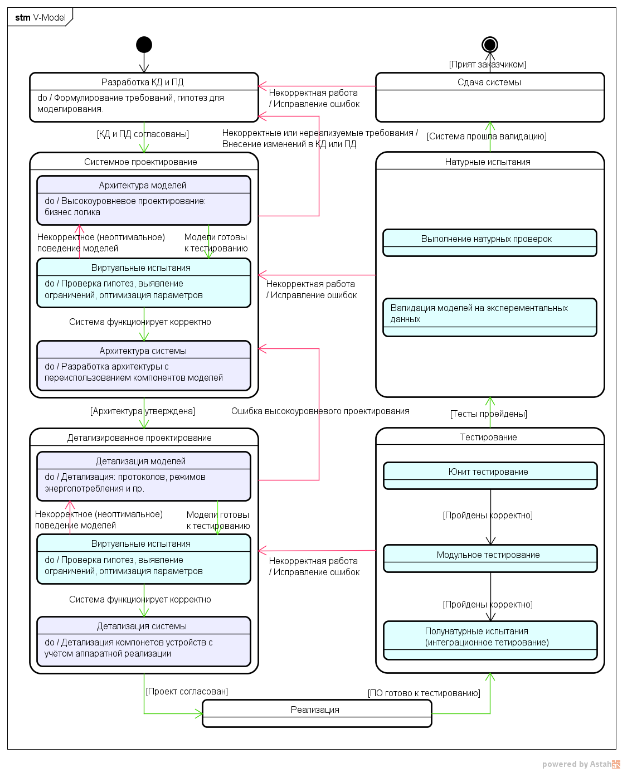
\includegraphics[
            width=\textwidth,
            height=0.8\textheight,
            keepaspectratio
        ]{./figures/modified_V-shaped_development_model.png}
        \caption{Модифицированная V-образная модель разработки}
        \label{fig:modified_V-shaped_development_model}
    \end{figure}

    \textbf{Разработка КД и ПД.}
    Цель этого этапа -- определение функциональных и нефункциональных требований к системе,
    разработка конструкторской и программной документации.
    На этой стадии формулируются гипотезы, которые впоследствии проверяются с помощью компьютерного моделирования.
    Такие проверки могут включать подбор оптимального числа агентов в системе,
    определение требуемой мощности излучателей, выбор наиболее эффективного протокола связи и другие параметры.
    Результаты моделирования позволяют оперативно согласовать спорные пункты технического задания,
    улучшить совокупные показатели системы за счёт правильного сочетания параметров и
    существенно снизить риск ошибок проектирования на более поздних стадиях разработки.

    \textbf{Системное проектирование.}
    Цель этого этапа -- создание архитектуры системы.
    На этой стадии разрабатываются компьютерные модели, направленные на проверку гипотез, сформулированных ранее.
    Их основная цель -- реализация ключевых функций агентов, без необходимости точного
    воспроизведения всех физических и аппаратных деталей.
    Даже такие упрощённые модели позволяют выявить потенциальные ограничения,
    оптимизировать параметры системы и, при необходимости, скорректировать техническое задание.

    \textbf{Детализированное проектирование.}
    Цель этого этапа -- описание модулей, классов, функций и их взаимодействий, ключевых алгоритмов и протоколов связи.
    На этапе детализированного проектирования, при необходимости,
    дополняются и уточняются элементы компьютерных моделей, разработанные на предыдущем этапе.
    Это позволяет более точно воспроизвести поведение системы,
    проверить не подтверждённые ранее гипотезы и выявить потенциальные проблемы до реализации реальных устройств.
    В частности, могут быть добавлены реализации протоколов связи, параметры используемых антенн,
    модели энергопотребления автономных подводных аппаратов и другие детали, повышающие достоверность моделирования.
    Такой подход способствует более точному прогнозированию поведения системы в сложных и критических условиях.

    \textbf{Тестирование.}
    Цель этого этапа -- проверка программного обеспечения с помощью юнит и модульных тестов,
    проведение лабораторных испытаний.
    Помимо юнит- тестирования, на данном этапе реализуется интеграционное тестирование в виде полунатурных испытаний,
    позволяющих оценить поведение системы в различных условиях.
    В ходе таких испытаний часть программных модулей заменяется их реальными аппаратными реализациями.
    Для проведения полунатурных испытаний разрабатывается специальный тестовый стенд,
    который может работать в следующих режимах:

    \begin{itemize}
        \item
        Полностью виртуальная среда, имитирующая внешнюю среду для тестируемых устройств
        (траектории движения, характеристики каналов связи и др.);
        \item
        Гибридная среда, включающая компьютерные модели приборов, компонентов и датчиков,
        взаимодействующих с реальными устройствами.
    \end{itemize}

    Такой подход позволяет моделировать сценарии, которые трудно достижимы в лабораторных условиях,
    а иногда экономически нецелесообразны при натурных испытаниях.
    К ним относятся:
    \begin{itemize}
        \item сценарии с большим количеством агентов, превышающим количество, доступное для натурного тестирования;
        \item сложные топологии сетей и взаимодействий между агентами системы;
        \item многократные сбои связи, задержки передачи данных и отказы в работе узлов;
        \item моделирование различных уровней заряда аккумуляторов и сценариев энергопотребления;
        \item сложные траектории движения и динамические изменения окружающей среды;
        \item
        исключительные ситуации, имеющие высокую степень риска или требующие значительных затрат
        (например, аварийные режимы, синхронные отказы и т.п.).
    \end{itemize}
    Использование тестового стенда обеспечивает возможность проведения большего количества проверок,
    более полной верификации алгоритмов управления, навигации и связи,
    а также выявление потенциальных сбоев до запуска реальных аппаратов в воде.
    Это позволяет повысить надёжность системы и \hl{потенциально} сократить общие затраты на натурные испытания.

    \textbf{Натурные испытания.}
    Цель этого этапа, проверка работы системы в реальных условиях эксплуатации.
    При проведении натурных испытаний на полигоне помимо проверки
    корректности функционирования системы и её отдельных компонентов
    появляется возможность провести валидацию разработанных ранее компьютерных моделей.
    Сравнение данных, полученных в ходе моделирования,
    с результатами натурных измерений позволяет оценить адекватность моделей
    и при необходимости внести коррективы в параметры симуляций или в саму архитектуру системы.

    Таким образом, применение компьютерного моделирования в рамках V-образной модели разработки
    не только повышает техническую надёжность системы, но и оптимизирует бизнес-процессы:
    сокращает сроки,
    снижает
    затраты,
    минимизирует риски и
    повышает качество конечного продукта.
    Моделирование становится ключевым элементом
    устойчивой и эффективной разработки сложных программно-аппаратных систем.


    \subsection{Постановка задачи моделирования на физическом уровне}
    \label{subsec:statement_of_modeling_problem_at_physical_level}

    В рамках настоящей работы моделирование на физическом уровне понимается
    как построение вычислительно эффективной модели,
    предназначенной для виртуальных испытаний программно-аппаратных гидроакустических приёмопередатчиков
    в составе мультиагентной системы.
    Разрабатываемая модель должна обеспечивать возможность оценки основных характеристик передачи сигнала между узлами,
    включая задержку распространения, ослабление сигнала в среде, влияние шумов и помех,
    а также факт успешного или неуспешного приёма пакета.
    При этом модель должна быть достаточно простой для использования в сетевом симуляторе,
    где требуется проведение большого числа вычислительных экспериментов.

    В работе реализуются две взаимосвязанные модели физического уровня:
    упрощённая модель гидроакустического канала связи и упрощённая модель гидроакустического приёмопередатчика.
    Первая модель описывает распространение сигнала от передатчика к приёмнику в водной среде и
    определяет задержку и энергетические потери сигнала.
    Вторая модель описывает режим работы узла связи при передаче и приёме,
    а также правило принятия решения о возможности успешного приёма сигнала на основе энергетического критерия.

    С целью обеспечения вычислительной эффективности и соответствия задачам сетевого моделирования
    в работе принимаются следующие допущения.
    Распространение сигнала рассматривается как однолучевое и осуществляется
    только по прямой от излучателя к приёмнику.
    Скорость звука в воде считается постоянной величиной.
    Потери при распространении учитывают только геометрическое расхождение волнового фронта и абсорбцию в среде.
    Сигнал рассматривается в одной рабочей полосе частот вокруг одной несущей частоты.
    Его описание выполняется в энергетическом представлении через спектральную плотность мощности,
    выражаемую в гидроакустических единицах давления, Па²/Гц.
    Приёмопередатчик работает в полудуплексном режиме,
    то есть одновременная передача и приём одним узлом не допускаются.
    Излучатель и приёмник в рамках данной модели считаются изотропными.
    Решение о приёме сигнала принимается по рассчитанному
    отношению мощности полезного сигнала к суммарной мощности шума и помех (далее SINR).

    Перечисленные допущения задают границы применимости модели.
    В реализуемом варианте не учитываются
    многолучёвость,
    отражения от поверхности и дна,
    рефракция,
    пространственная изменчивость скорости звука,
    эффект Доплера,
    фазовая структура сигнала и детальные процессы
    электроакустического преобразования внутри аппаратного тракта.
    Таким образом, модель не претендует на полное физическое воспроизведение гидроакустической среды,
    а ориентирована на описание тех факторов,
    которые являются существенными для сетевого моделирования передачи пакетов между узлами.

    С формальной точки зрения входными данными модели канала связи являются координаты передатчика и приёмника,
    а также параметры излучаемого сигнала в заданной рабочей полосе частот.
    Выходными данными модели канала являются
    задержка распространения и
    спектральная плотность мощности сигнала на входе приёмника с учётом потерь в среде.
    Входными данными модели приёмопередатчика являются спектральная плотность мощности полезного сигнала,
    а также спектральные плотности мощности шума и помех в рабочей полосе.
    Выходом модели приёмопередатчика является рассчитанное значение SINR и
    решение об успешном или неуспешном приёме пакета.

    Выбранный уровень абстракции позволяет сосредоточиться на тех свойствах физического уровня,
    которые являются определяющими для рассматриваемой задачи:
    задержке распространения,
    энергетическом ослаблении сигнала,
    влиянии шума и взаимных помех,
    а также возможности корректного приёма при совместной работе нескольких узлов.
    В дальнейшем на этой основе формулируются
    формальная модель гидроакустического канала связи и
    формальная модель гидроакустического приёмопередатчика,
    непосредственно используемые при реализации компьютерной модели.


    \subsection{Формальная модель гидроакустического канала связи}
    \label{subsec:Formal_model_of_hydroacoustic_communication_channel}

    В рамках настоящей работы гидроакустический канал связи рассматривается как среда,
    которая преобразует излучаемый сигнал в принимаемый за счёт
    конечной скорости распространения звука и
    энергетических потерь.
    Поскольку в реализуемой модели принято однолучевое распространение по прямой между передатчиком и приёмником,
    формальная модель канала сводится к вычислению
    расстояния между узлами,
    задержки распространения сигнала,
    потерь на геометрическое расхождение и потерь на абсорбцию.
    Результатом работы модели канала являются
    задержка прихода сигнала и
    спектральная плотность мощности сигнала на входе приёмника.

    Расстояние между передатчиком и приёмником определяется как евклидово
    расстояние между их координатами (см.~формулу~\eqref{eq:euclidean_distance}):
    \begin{equation}
        d = \left\| r_{rx} - r_{tx} \right\|
        \label{eq:euclidean_distance}
    \end{equation}
    \begin{FqwWhere}
        \(d\) -- расстояние между передатчиком и приёмником;\\
        \(r_{tx}\) -- радиус-вектор передатчика;\\
        \(r_{rx}\) -- радиус-вектор приёмника.
    \end{FqwWhere}

    Поскольку скорость звука в среде в настоящей работе принимается постоянной,
    задержка распространения сигнала определяется выражением (см.~формулу~\eqref{eq:propagation_delay}):
    \begin{equation}
        \tau = \frac{d}{c}
        \label{eq:propagation_delay}
    \end{equation}
    \begin{FqwWhere}
        \(\tau\) -- задержка распространения сигнала, с.;\\
        \(d\) -- расстояние между передатчиком и приёмником, м.;\\
        \(c\) -- скорость звука в воде, м/с.
    \end{FqwWhere}

    Для описания ослабления сигнала в канале используются суммарные потери передачи,
    включающие потери на геометрическое расхождение и потери на абсорбцию.
    В общем виде это записывается следующим образом (см.~формулу~\eqref{eq:propagation_loss}):
    \begin{equation}
        TL(f,d) = {TL}_{geom}(d) + {TL}_{abs}(f,d)
        \label{eq:propagation_loss}
    \end{equation}
    \begin{FqwWhere}
        \(TL\) (Transmission loss) -- суммарные потери сигнала на частоте \(f\) при расстоянии \(d\), дБ;\\
        \({TL}_{geom}\) -- потери на геометрическое расхождение, дБ;\\
        \({TL}_{abs}\) -- потери на абсорбцию, дБ;\\
        \(f\) -- частота сигнала, Гц;\\
        \(d\) -- расстояние, пройденное сигналом, м.
    \end{FqwWhere}

    При распространении акустической волны её энергия распределяется по всё большей площади волнового фронта,
    что приводит к уменьшению плотности энергии сигнала с расстоянием.
    В инженерной форме потери на геометрическое расхождение принято задавать выражением
    (см.~формулу~\eqref{eq:loss_of_geometric_divergence}):
    \begin{equation}
        {TL}_{geom}(d) = 10n\log_{10}d
        \label{eq:loss_of_geometric_divergence}
    \end{equation}
    \begin{FqwWhere}
        \({TL}_{geom}\) -- потери на геометрическое расхождение, дБ;\\
        \(n\) -- коэффициент расхождения;\\
        \(d\) -- расстояние, пройденное сигналом, м.
    \end{FqwWhere}

    Значение коэффициента n определяет тип расхождения волнового фронта.
    При n~=~2 реализуется \emph{сферическое расхождение}, характерное для распространения волны в свободном объёме.
    При n~=~1 реализуется \emph{цилиндрическое расхождение}, соответствующее распространению в ограниченном слое.
    В общем случае могут использоваться промежуточные эмпирические значения коэффициента n,
    позволяющие учитывать условия распространения без усложнения модели.

    Помимо геометрического расхождения, при распространении акустического сигнала в водной среде
    возникают потери на абсорбцию, обусловленные необратимым преобразованием части акустической энергии в тепловую.
    В реализуемой модели эта составляющая задаётся как
    (см.~формулу~\eqref{eq:absorption_loss}):
    \begin{equation}
        {TL}_{abs}(f,d) = \alpha(f) \cdot d \cdot 10^{3}
        \label{eq:absorption_loss}
    \end{equation}
    \begin{FqwWhere}
        \({TL}_{abs}\) -- потери на абсорбцию, дБ;\\
        \(\alpha\) -- коэффициент поглощения, дБ/км;\\
        \(d\) -- расстояние, пройденное сигналом, м.
    \end{FqwWhere}

    Для вычисления коэффициента абсорбции в работе используются формулы
    Торпа (см.~формулу~\eqref{eq:thorp_absorption}) и
    формула Франсуа-Гаррисона (см.~формулу~\eqref{eq:francois_garrison_absorption}):
    \begin{equation}
        \alpha(f) \approx
        \frac{0.11f^{2}}{1 + f^{2}} +
        \frac{40f^{2}}{4100 + f^{2}} +
        \frac{0,03f^{2}}{36 + f^{2}}
        \label{eq:thorp_absorption}
    \end{equation}
    \begin{FqwWhere}
        \(\alpha\) -- коэффициент поглощения, дБ/км;\\
        \(f\) -- частота звука, кГц.
    \end{FqwWhere}

    \begin{equation}
        \begin{aligned}
            \alpha(f) \approx{}&
            \frac{A_{1}P_{1}f_{1}f^{2}}{f_{1}^{2} + f^{2}} +
            \frac{A_{2}P_{2}f_{2}f^{2}}{f_{2}^{2} + f^{2}} +
            A_{3}P_{3}f^{2},\\
            A_{1} ={}& \frac{8.86}{c} \cdot {10}^{0.78pH - 5},\quad P_{1} = 1,\\
            f_{1} ={}& 2.8\sqrt{\frac{S}{35}} \cdot 10^{4 - \frac{1245}{273 + T}},\\
            A_{2} ={}& 21.44\frac{S}{c}(1 + 0.025T),\\
            P_{2} ={}& 1 - 1.37 \cdot 10^{-4}D + 6.2 \cdot 10^{-9}D^{2},\\
            f_{2} ={}& \frac{8.17 \cdot 10^{8 - \frac{1990}{273 + T}}}{1 + 0.0018(S - 35)},\\
            A_{3} ={}&
            \begin{cases}
                4.937 \cdot 10^{-4} - 2.59 \cdot 10^{-5}T +
                9.11 \cdot 10^{-7}T^{2} - 1.50 \cdot 10^{-8}T^{3}, & T \geq 20,\\
                3.964 \cdot 10^{-4} - 1.146 \cdot 10^{-5}T +
                1.45 \cdot 10^{-7}T^{2} - 6.5 \cdot 10^{-10}T^{3}, & T < 20,
            \end{cases}\\
            P_{3} ={}& 1 - 3.83 \cdot 10^{-5}D + 4.9 \cdot 10^{-10}D^{2},\\
            c ={}& 1412 + 3.21T + 1.19S + 0.0167D
        \end{aligned}
        \label{eq:francois_garrison_absorption}
    \end{equation}
    \begin{FqwWhere}
        \(\alpha\) -- коэффициент поглощения, дБ/км;\\
        \(f\) -- частота звука, кГц;\\
        \(A_{1}\) -- амплитудный коэффициент вклада борной кислоты;\\
        \(A_{2}\) -- амплитудный коэффициент вклада сульфата магния;\\
        \(A_{3}\) -- амплитудный коэффициент вклада чистой воды;\\
        \(P_{1},\ P_{2},\ P_{3}\) -- поправочные множители на давление/глубину;\\
        \(f_{1}\) -- релаксационная частота борной кислоты, кГц;\\
        \(f_{2}\) -- релаксационная частота сульфата магния, кГц;\\
        \(T\) -- температура воды, °C;\\
        \(S\) -- солёность, ‰;\\
        \(D\) -- глубина, м;\\
        \(pH\) -- водородный показатель воды;\\
        \(c\) -- скорость звука в воде, м/с.
    \end{FqwWhere}

    \hl{}

    Формулы~\eqref{eq:thorp_absorption} и~\eqref{eq:francois_garrison_absorption}
    задают инженерную аппроксимацию частотной зависимости абсорбции и
    позволяет учитывать увеличение потерь при росте частоты сигнала.

    В модели сигнал описывается через спектральную плотность мощности на выходе передатчика \(S_{tx}(f)\),
    измеряемую в Па²/Гц.
    Тогда спектральная плотность мощности сигнала на входе приёмника определяется выражением
    (см.~формулу~\eqref{eq:received_power_spectral_density}):
    \begin{equation}
        S_{rx} = S_{tx} \cdot 10^{-\frac{TL(f)}{10}}
        \label{eq:received_power_spectral_density}
    \end{equation}
    \begin{FqwWhere}
        \(S_{rx}\) -- спектральная плотность мощности сигнала на входе приёмника, Па²/Гц;\\
        \(S_{tx}\) -- спектральная плотность мощности сигнала на выходе передатчика, Па²/Гц;\\
        \(TL\) (Transmission loss) -- суммарные потери передачи, дБ;\\
        \(f\) -- частота сигнала, Гц;\\
        \(d\) -- расстояние, пройденное сигналом, м.
    \end{FqwWhere}

    Выражение~\eqref{eq:received_power_spectral_density} задаёт основное преобразование,
    выполняемое моделью канала связи.
    Таким образом, по заданным координатам узлов и параметрам сигнала
    модель канала позволяет определить две ключевые величины, используемые далее в модели приёмопередатчика:
    задержку распространения τ и
    спектральную плотность мощности принятого сигнала~S\textsubscript{rx}(f).


    \subsection{Формальная модель гидроакустического приёмопередатчика}
    \label{subsec:formal_model_of_hydroacoustic_transceiver}

    В рамках настоящей работы гидроакустический приёмопередатчик рассматривается как узел сети,
    функционирующий на физическом уровне в упрощённом энергетическом представлении.
    Такая модель не описывает внутреннюю аппаратную структуру устройства на уровне отдельных электронных компонентов,
    а задаёт формальные правила его работы при передаче и приёме сигналов в гидроакустическом канале связи.
    Основное назначение данной модели состоит в определении условий, при которых сигнал,
    поступающий на вход приёмника, может быть успешно принят в присутствии шумов и помех.

    В реализуемой модели приёмопередатчик работает в полудуплексном режиме.
    Это означает, что один и тот же узел в каждый момент времени может либо передавать сигнал, либо принимать его,
    но не выполнять эти действия одновременно.
    Следовательно, в интервале собственной передачи узел не рассматривается как доступный для приёма внешних сигналов.

    Излучающие и приёмные свойства узла в данной работе задаются в упрощённом виде.
    Передающая и приёмная части считаются изотропными, то есть направленные характеристики антенн не учитываются.
    В рамках принятой модели это означает, что мощность сигнала определяется только параметрами излучения,
    рабочей полосой частот и потерями в канале связи,
    а пространственная направленность преобразователей не вносит дополнительного вклада
    в расчёт уровня сигнала на приёмной стороне.

    Полезный сигнал на входе приёмника задаётся через спектральную плотность мощности,
    определённую формулой~\eqref{eq:received_power_spectral_density}.
    Полезная мощность сигнала в рабочей полосе частот {[}f\textsubscript{1},f\textsubscript{2}{]}
    вычисляется интегрированием спектральной плотности мощности по этой полосе
    (см.~формулу~\eqref{eq:useful_signal_power}):
    \begin{equation}
        P_{s} = \int_{f_{1}}^{f_{2}} S_{rx}(f) df
        \label{eq:useful_signal_power}
    \end{equation}
    \begin{FqwWhere}
        \(P_{s}\) -- мощность полезного сигнала в рабочей полосе, Па²;\\
        \(f_{1}\) -- нижняя граница рабочей полосы, Гц;\\
        \(f_{2}\) -- верхняя граница рабочей полосы, Гц;\\
        \(S_{rx}\) -- спектральная плотность мощности полезного сигнала на входе приёмника, Па²/Гц.
    \end{FqwWhere}

    Помимо полезного сигнала, на входе приёмника присутствуют шум и помехи от других одновременных передач.
    В рамках принятой модели они учитываются также в энергетическом представлении через спектральные плотности мощности
    (см.~формулы~\eqref{eq:noise_power} и~\eqref{eq:interference_power}):
    \begin{equation}
        P_{n} = \int_{f_{1}}^{f_{2}} S_{n}(f) df
        \label{eq:noise_power}
    \end{equation}
    \begin{equation}
        P_{i} = \int_{f_{1}}^{f_{2}} S_{i}(f) df
        \label{eq:interference_power}
    \end{equation}
    \begin{FqwWhere}
        \(P_{n}\) -- мощность шума в рабочей полосе, Па²;\\
        \(S_{n}\) -- спектральная плотность мощности шума, Па²/Гц;\\
        \(P_{i}\) -- мощность помехи (другого сигнала) в рабочей полосе, Па²;\\
        \(S_{i}\) -- спектральная плотность мощности помехи на входе приёмника, Па²/Гц.
    \end{FqwWhere}

    Критерием успешного приёма в модели является отношение мощности полезного сигнала к суммарной мощности шума и помех.
    Для этого используется величина SINR, определяемая выражением
    (см.~формулу~\eqref{eq:sinr}):
    \begin{equation}
        SINR = \frac{P_{s}}{\sum_{k = 1}^{N_{i}}\left(P_{i,k}\right) + P_{n}}
        \label{eq:sinr}
    \end{equation}
    \begin{FqwWhere}
        \(SINR\) -- отношение мощности полезного сигнала к суммарной мощности шума и помех;\\
        \(P_{s}\) -- мощность полезного сигнала в рабочей полосе, Па²;\\
        \(P_{n}\) -- мощность шума в рабочей полосе, Па²;\\
        \(N_{i}\) -- число мешающих передач (других сигналов);\\
        \(P_{i,k}\) -- мощность k-й помехи (другого сигнала) в рабочей полосе, Па².
    \end{FqwWhere}

    Решение о возможности успешного приёма пакета принимается путём сравнения
    расчётного значения SINR
    с заданным порогом приёма γ\textsubscript{th}.
    Если выполняется условие (см.~формулу~\eqref{eq:successful_reception_condition}):
    \begin{equation}
        SINR \geq \gamma_{th}
        \label{eq:successful_reception_condition}
    \end{equation}
    \begin{FqwWhere}
        \(SINR\) -- отношение мощности полезного сигнала к суммарной мощности шума и помех;\\
        \(\gamma_{th}\) -- порог успешного приёма.
    \end{FqwWhere}

    то пакет считается успешно принятым.
    В противном случае пакет считается потерянным.

    Таким образом, формальная модель гидроакустического приёмопередатчика в
    настоящей работе задаёт правила функционирования узла в полудуплексном режиме,
    определяет способ представления полезного сигнала, шумов и помех в виде спектральных плотностей мощности и
    формулирует критерий успешного приёма сигнала на основе отношения SINR.
    В сочетании с моделью канала связи, рассмотренной в пункте 2.3,
    это образует завершённую математическую основу реализуемой модели физического уровня.

    \subsection*{Выводы}\label{subsec:conclusions_of_chapter_2}
    \addcontentsline{toc}{section}{Выводы}

    Во втором разделе была рассмотрена интеграция компьютерного моделирования в
    V-образную модель разработки программно-аппаратных гидроакустических систем.
    Показано, что включение этапов виртуальных испытаний в общий процесс проектирования
    позволяет перенести проверку части технических решений на более ранние стадии разработки.
    Это снижает зависимость от дорогостоящих натурных испытаний,
    уменьшает риск позднего выявления критических ошибок и
    делает процесс разработки более управляемым.

    Далее была сформулирована постановка задачи моделирования на физическом уровне.
    В рамках настоящей работы в качестве реализуемого решения выбраны упрощённая модель гидроакустического канала связи
    и упрощённая модель гидроакустического приёмопередатчика.
    Принятые допущения ориентированы на обеспечение вычислительной эффективности модели и
    её пригодности для использования в сетевом симуляторе при проведении виртуальных испытаний мультиагентных систем.

    В разделе также построена формальная модель
    гидроакустического канала связи и
    гидроакустического приёмопередатчика.
    В результате были определены основные параметры и соотношения, необходимые для описания передачи сигнала,
    его ослабления при распространении и оценки условий успешного приёма пакета.
    Тем самым была сформирована математическая основа предлагаемого решения,
    непосредственно связанная с задачами настоящей работы.

    Полученные результаты образуют теоретическую и математическую основу
    для дальнейшего проектирования структуры компонентов программной модели и её
    реализации в следующем разделе.
    В то же время принятая постановка сохраняет возможности дальнейшего расширения системы
    за счёт добавления более сложных моделей канала и приёмопередатчиков,
    включая многолучёвое распространение,
    переменный профиль скорости звука,
    учёт эффекта Доплера,
    направленные характеристики преобразователей и
    более сложные механизмы обработки сигналов и
    правил принятия решения о приёме.


    \section{Проектирование и разработка модуля гидроакустической связи}\label{sec:module_design}

    \subsection{Требования к компьютерным моделям}
    \label{subsec:requirements_for_models}

    На основе проведённого анализа предметной области, существующих решений и формальных моделей,
    представленных во второй главе,
    в этом разделе сформулированы функциональные и нефункциональные требования к компьютерным моделям.
    В рамках работы планируется реализовать две взаимосвязанные модели:
    модель гидроакустического канала связи и модель программно-аппаратного гидроакустического приёмопередатчика.
    Обе модели проектируются с учётом принципов
    модульности,
    гибкости настройки и
    совместимости с сетевым симулятором Ns-3.

    Функциональные требования к компьютерной модели гидроакустического
    приёмопередатчика:

    \begin{enumerate}
        \def\labelenumi{\arabic{enumi}.}
        \item
        Модель приёмопередатчика должна обеспечивать взаимодействие с моделью
        гидроакустического канала связи;
        \item
        Модель приёмопередатчика работает в полудуплексном режиме, то есть
        приёмопередатчик не может осуществлять приём и передачу сигнала
        одновременно;
        \item
        Модель приёмопередатчика должна осуществлять отправку информационных
        акустических сигналов в модель канала связи;
        \item
        Модель приёмопередатчика должна осуществлять приём информационных
        акустических сигналов из модели канала связи и принимать решение о
        качестве приёма сигнала;
        \item
        Модель приёмопередатчика должна принимать пакет от вышестоящего уровня
        (по модели OSI), добавлять к нему простой MAC заголовок и
        конвертировать сигнал в акустический для отправки в канал связи;
        \item
        MAC-заголовок должен содержать MAC-адрес отправителя и получателя;
        \item
        Модель приёмопередатчика должна декодировать акустический сигнал в
        информационный пакет, затем декодировать MAC заголовок и передавать
        пакет, без MAC заголовка, на вышестоящий уровень;
        \item
        Модель передаёт пакет на верхний уровень только в случае совпадения
        MAC-адреса получателя в заголовке c MAC-адресом данного
        приёмопередатчика;
        \item
        Модель приёмопередатчика должна иметь FIFO очередь пакетов на входе
        физического уровня;
    \end{enumerate}

    Нефункциональные требования к компьютерной модели гидроакустического
    приёмопередатчика:

    \begin{enumerate}
        \def\labelenumi{\arabic{enumi}.}
        \item
        Модель гидроакустического приёмопередатчика должна быть спроектирована
        с потенциальной поддержкой различных моделей гидроакустических канала
        связи;
        \item
        Модель приёмопередатчика должна иметь порог обнаружения сигнала,
        представленный в виде спектральной плотности мощности в Па\^{}2/Гц.
        Сигналы ниже данного порога не обрабатываются моделью;
        \item
        Модель приёмопередатчика должна принимать решение о качестве
        принимаемого сигнала (принят / не принят) на основе порогового
        значения SINR (формула~\eqref{eq:sinr});
        \item
        MAC-адрес должен состоять из 8 бит.
        \item
        Акустический сигнал приёмопередатчика описывается спектральной
        плотностью мощности (Па\^{}2/Гц) и длительностью сигнала;
        \item
        Модель позволяет настраивать параметры: порог приёма, порог
        обнаружения, MAC-адрес узла.
    \end{enumerate}

    Функциональные требования к компьютерной модели гидроакустического
    канала связи:

    \begin{enumerate}
        \def\labelenumi{\arabic{enumi}.}
        \item
        Модель канал связи должна осуществлять распространение акустических
        сигналов между моделями гидроакустических приёмопередатчиков.
    \end{enumerate}

    Нефункциональные требования к компьютерной модели гидроакустического
    канала связи:

    \begin{enumerate}
        \def\labelenumi{\arabic{enumi}.}
        \item
        Модель должна определять задержку распространения сигнала на основе
        расстояния между узлами и скорости звука в воде (см.~формулу~\eqref{eq:propagation_delay});
        \item
        Модель позволяет настраивать постоянное значение скорости звука в
        среде;
        \item
        Модель должна вычислять суммарные потери сигнала согласно формуле
        (см.~формулу~\eqref{eq:propagation_loss}), с учётом геометрического расхождения
        (см.~формулу~\eqref{eq:loss_of_geometric_divergence}) и потерь на абсорбцию в среде по формуле Торпа
        (см.~формулы~\eqref{eq:absorption_loss} и~\eqref{eq:thorp_absorption});
        \item
        Модель позволяет настраивать коэффициент n из формулы расчёта потерь
        на геометрическое расхождение (см.~формулу~\eqref{eq:loss_of_geometric_divergence}).
        \item
        Модель гидроакустического канала связи должна осуществлять
        распространение акустических сигналов с учётом времени распространения
        и потерь распространения (формулы~\eqref{eq:euclidean_distance}--\eqref{eq:francois_garrison_absorption});
        \item
        Модель выполняет расчёт спектральной плотности мощности сигнала на
        входе приёмника (Па\^{}2/Гц).
    \end{enumerate}

    Общие нефункциональные требования к разрабатываемым моделям:

    \begin{enumerate}
        \def\labelenumi{\arabic{enumi}.}
        \item
        Модели должны поддерживать систему атрибутов Ns-3 для конфигурирования
        параметров без необходимости модификации исходного кода;
        \item
        Настройка сценариев моделирования осуществляется через скрипты на
        языке C++;
        \item
        Модели должны быть реализованы с использованием модульной архитектуры
        в соответствии с принципами SOLID;
        \item
        В структуре компонентов должны быть предусмотрены базовые и
        абстрактные классы, позволяющие разработчикам реализовывать
        собственные модели на их основе;
        \item
        Должны быть определены чёткие интерфейсы взаимодействия между
        компонентами модели, позволяющие заменять отдельные части системы без
        модификации остального кода.
        \item
        Разработка компьютерных моделей, должна быть выполнена в формате
        гидроакустического модуля в Ns-3.
    \end{enumerate}

    3.2 Варианты использования компьютерных моделей

    Диаграмма вариантов использования гидроакустического модуля для
    моделирования программно-аппаратных гидроакустических приёмопередатчиков
    представлена на рисунке 3.1.

    Рисунок 3.1 -- диаграмма вариантов использования

    Диаграмма отражает основные сценарии взаимодействия пользователя с
    разрабатываемой моделью. Варианты использования включают настройку
    параметров, запуск симуляции, получение и анализ результатов.


    \section*{3.2 Структура компонентов компьютерных
    моделей}\label{ux441ux442ux440ux443ux43aux442ux443ux440ux430-ux43aux43eux43cux43fux43eux43dux435ux43dux442ux43eux432-ux43aux43eux43cux43fux44cux44eux442ux435ux440ux43dux44bux445-ux43cux43eux434ux435ux43bux435ux439}
    \addcontentsline{toc}{section}{3.2 Структура компонентов компьютерных
    моделей}

    Модель гидроакустического приёмопередатчика должна быть спроектирована в
    соответствии с сетевой моделью OSI. Как уже было сказано в пункте 1.2,
    приёмопередатчик реализует канальный и физический уровень. В общем
    случае, модель гидроакустического приёмопередатчика описывается с
    помощью следующей диаграммы классов (см.~рисунок~3.1).

    Рисунок 3.1 -- диаграмма классов общей модели гидроакустического
    приёмопередатчика

    На диаграмме классов общей модели гидроакустического приёмопередатчика
    представлены следующие классы:

    \begin{itemize}
        \item
        \textbf{NetDevice} -- стандартный интерфейс сетевых устройств в Ns-3.
        Описывает контракт, который должны реализовывать сетевые устройства;
        \item
        \textbf{Channel} -- стандартный интерфейс каналов связи в Ns-3.
        Предоставляет абстрактные методы для доступа к сетевым устройствам
        NetDevice;
        \item
        \textbf{HaNetDevice} -- абстрактный класс, являющийся специализацией
        сетевого устройства для моделей программно-аппаратного
        гидроакустического приёмопередатчика. Он предоставляет доступ к
        классам, описывающим физический уровень приёмопередатчика, и
        осуществляет их настройку. Наследники этого класса определяют
        поведение приёмопередатчика на 2 уровне модели OSI;
        \item
        \textbf{HaPhyBehavior} -- абстрактный класс, реализующий поведение
        приёмопередатчика на 1 уровне модели OSI. Класс организует
        взаимодействие с MAC уровнем через HaNetDevice и с каналом связи через
        класс HaPhy;
        \item
        \textbf{HaPhy} -- абстрактный класс физического уровня
        приёмопередатчика, предоставляющий методы для отправки и приёма
        акустических сигналов. Наследники этого класса определяют особенности
        работы с конкретными моделями гидроакустических каналов связи.
    \end{itemize}

    Компоновка классов таким образом, позволяет использовать модель
    приёмопередатчика как сетевое устройство в симуляциях Ns-3 (за счёт
    стандартного интерфейса NetDevice), позволяет реализовывать различное
    поведение на канальном и физическом уровнях (благодаря использованию
    HaNetDevice и HaPhyBehavior), а также позволяет использовать модели
    приёмопередатчиков с различными моделями каналов связи (за счёт
    абстрактного класса HaPhy). Эта компоненты является главным каркасом для
    создания моделей программно-аппаратных гидроакустических
    приёмопередатчиков.

    Важной частью любой системы связи являются данные, передаваемые
    устройствами по сети. В разрабатываемой системе моделирования их место в
    системе отображено на следующей диаграмме классов (см.~рисунок~3.2).

    Рисунок 3.2 -- диаграмма классов пакетов в модели гидроакустического
    приёмопередатчика

    На диаграмме классов пакетов в модели гидроакустического
    приёмопередатчика представлены следующие классы:

    \begin{itemize}
        \item
        \textbf{Packet} -- стандартный класс в Ns-3, описывающий полезную
        информацию сетевых пакетов в симуляции;
        \item
        \textbf{HaMpdu} (mac protocol data unit) -- абстрактный класс,
        описывающий пакет MAC уровня. Хранит данные от вышестоящего уровня и
        предоставляет абстрактные методы для MAC-адресов отправителя и
        получателя;
        \item
        \textbf{HaPpdu} (physical protocol data unit) -- класс хранит
        передаваемую информацию и описывает физические параметры акустического
        сигнала;
        \item
        \textbf{HaTransmissionParameters} -- класс хранит физические параметры
        акустического сигнала в момент его излучения (отправки);
        \item
        \textbf{HaSignalType} -- класс-перечисление, описывающий тип сигнала.
    \end{itemize}

    Компоновка классов таким образом обеспечивает взаимодействие с
    вышестоящими уровнями протоколов связи через стандартный класс Packet и
    вносит необходимую специфику акустического сигнала через класс с
    параметрами HaTransmissionParameters.

    Основные функции гидроакустического приёмопередатчика на физическом
    уровне -- это преобразование акустических сигналов. Для выполнения этих
    операций в компьютерную модель приёмопередатчика вводятся следующие
    классы, представленные на диаграмме классов (см.~рисунок~3.3).

    Рисунок 3.3 -- диаграмма классов преобразователей акустических сигналов

    На диаграмме классов преобразователей акустических сигналов представлены
    следующие классы:

    \begin{itemize}
        \item
        \textbf{HaPpduDecoder} -- интерфейс устройства обработки и
        декодирования акустических сигналов описанных через HaPpdu;
        \item
        \textbf{HaMpduToPpduConverter} -- интерфейс формирователя
        акустического сигнала из пакета MAC уровня;
        \item
        \textbf{HaPpduProcessor} -- абстрактный класс, осуществляющий полную
        обработку акустических сигналов (декодирования и формирования) с
        использованием модели интерференции;
        \item
        \textbf{HaPpduPreamblePayloadProcessor} -- абстрактный класс
        осуществляющий приём акустических сигналов, начинающихся с преамбулы.
    \end{itemize}

    Процесс приёма сигнала в модели HaPpduPreamblePayloadProcessor
    представлен на следующей диаграмме последовательности (см.~рисунок~3.4).

    Рисунок 3.4 -- диаграмма последовательности приёма сигнала в
    HaPpduPreamblePayloadProcessor

    Благодаря сформулированным интерфейсам преобразователей, пользователи
    модуля смогут проектировать собственные решения, с учётом специфики
    других приёмопередатчиков, а в случае с HaPpduPreamblePayloadProcessor
    позволит быстро определить критерии приёма для конкретной структуры
    сигнала.

    Как уже упоминалось ранее, класс HaPpduProcessor использует модель
    интерференции. Она используется для рассчёта характеристик принимаемых
    сигналов. Диаграмма классов, описывающая компоненты модели интерференции
    представлена ниже (см.~рисунок~3.5).

    Рисунок 3.5 -- диаграмма классов модели интерференции

    На диаграмме классов модели интерференции представлены следующие классы:

    \begin{itemize}
        \item
        \textbf{HaInterferenceModel} -- интерфейс модели интерференции,
        осуществляющей сбор всех принимаемых сигналов и рассчёт характеристик
        приёма.
        \item
        \textbf{HaInterferenceStatus} -- интерфейс, предоставляющий
        рассчитанные характеристики приёма для сигнала.
        \item
        \textbf{HaInterferenceOneBandModel} -- модель интерференции,
        осуществляющая расчёт характеристик приёма для сигналов, описываемых
        одной частотной полосой.
        \item
        \textbf{HaInterferenceStatusTracker} -- класс, осуществляющий расчёт
        характеристик приёма сигнала с течением времени.
        \item
        \textbf{PsdOneBand} -- вспомогательный класс для
        HaInterferenceOneBandModel, который хранит информацию о спектральной
        плотности мощности сигнала в одной полосе частот.
        \item
        \textbf{PsdOneBandWithStatus} -- вспомогательный класс для
        HaInterferenceOneBandModel, который хранит статус сигнала и его
        информацию о спектральной плотности мощности в одной полосе частот.
    \end{itemize}

    Таким образом с помощью сформулированных интерфейсов HaInterferenceModel
    и HaInterferenceStatus пользователи модуля смогут реализовывать
    собственные модели интерференции. Для разрабатываемой модели
    приёмопередатчика используется модель интерференции
    HaInterferenceOneBandModel. Работа этой модели, представлена на
    диаграммах последовательностей (см.~рисунки~3.6-3.8).

    Рисунок 3.6 -- диаграмма последовательности приёма нового
    информационного сигнала в модель интерференции
    HaInterferenceOneBandModel

    Рисунок 3.7 -- диаграмма последовательности нового сигнала в модель
    интерференции HaInterferenceOneBandModel

    Рисунок 3.8 -- диаграмма последовательности обновления статусов сигналов
    в модели интерференции HaInterferenceOneBandModel

    Рассчёт характеристик в модели интерференции HaInterferenceOneBandModel
    осуществляется на основании мощности сигнала в одной полосе частот. Для
    рассчёта SNR используются формулы~\eqref{eq:received_power_spectral_density}--\eqref{eq:interference_power}.

    Связь поведения физического уровня с гидроакустическими
    преобразователями представлена на следующей диаграмме классов
    (см.~рисунок~3.9).

    Рисунок 3.9 -- диаграмма классов поведений физического уровня с
    акустическими преобразователями

    На диаграмме классов поведений физического уровня с их акустическими
    преобразователями представлены следующие классы:

    \begin{itemize}
        \item
        \textbf{HaPhyBehaviorPpduProcessorPerType} -- абстрактный класс
        поведения физического уровня. Хранит акустические преобразователи в
        соответствии их типу сигнала. Имеет общую модель интерференции со
        всеми акустическими преобразователями;
        \item
        \textbf{HaPhyBehaviorOneActiveSignalProcessor} -- абстрактный класс
        поведения физического уровня, предоставляющий один активный
        акустический преобразователь.
    \end{itemize}

    Работа приёмопередатчика в полудуплексном режиме описывается с помощью
    диаграммой машины состояний (см~рисунок~3.10) и диаграммы классов
    (см.~рисунок~3.11)

    Рисунок 3.10 -- диаграмма машины состояний модели приёмопередатчика в
    полудуплексном режиме

    На диаграмме машины состояний модели приёмопередатчика в полудуплексном
    режиме представлены следующие состояния:

    \begin{itemize}
        \item
        \textbf{Off} -- устройство отключено;
        \item
        \textbf{IDLE} -- устройство находится в режиме ожидания входящих и
        исходящих сигналов;
        \item
        \textbf{Tx} -- устройство находится в режиме отправки акустического
        сигнала;
        \item
        \textbf{Rx} -- устройство находится в режиме приёма акустического
        сигнала.
    \end{itemize}

    Рисунок 3.11 -- диаграмма классов машины состояний модели
    приёмопередатчика

    На диаграмме классов поведений физического уровня с их акустическими
    преобразователями представлены следующие классы:

    \begin{itemize}
        \item
        \textbf{TransceiverStateMachineType} -- класс-перечисление,
        описывающий состояние приёмопередатчика.
        \item
        \textbf{TransceiverStateMachine} -- базовый класс машины состояний
        приёмопередатчика.
    \end{itemize}

    Конечное поведение модели приёмопередатчика описывается классами,
    представленными на следующей диаграмме классов (см.~рисунок~3.12).

    Рисунок 3.12 -- диаграмма классов модели гидроакустического
    приёмопередатчика

    На диаграмме классов модели гидроакустического приёмопередатчика
    представлены следующие классы:

    \begin{itemize}
        \item
        \textbf{SimpleHaNetDevice} -- класс сетевого устройства, определяющий
        поведение модели гидроакустического приёмопередатчика на канальном
        уровне. Содержит простейшую MAC очередь (HaMpduQueue);
        \item
        \textbf{HaMpduQueue} -- класс очереди пакетов MAC уровня. Хранит
        пакеты, подготовленные к отправке, и передаёт их на физических
        уровень, когда тот готов передавать;
        \item
        \textbf{SimpleHaMpdu} -- класс пакета MAC уровня, содержащий
        восьмибитные адреса отправителя и получателя;
        \item
        \textbf{SimpleHaPhyBehavior} -- класс поведение физического уровня
        модели приёмопередатчка, осуществляющее работу в полудуплексном
        режиме;
        \item
        \textbf{SimplePpduProcessor} -- класс обработчика акустических
        сигналов, определяющий правила кодирования и декодирования сигналов с
        преамбулой.
    \end{itemize}

    Процесс отправки пакета на канальном уровне в модели гидроакустического
    приёмопередатчика представлен на следующих диаграммах последовательности
    (см.~рисунок~3.13, 3.14).

    Рисунок 3.13 -- диаграмма последовательности отправки нового пакета на
    канальном уровне

    Рисунок 3.14 -- диаграмма последовательности взаимодействия очереди с
    поведением физического уровня

    Процесс отправки пакета на физическом уровне модели гидроакустического
    приёмопередатчика представлен на следующих диаграммах последовательности
    (см.~рисунок~3.15).

    Рисунок 3.15 -- диаграмма последовательности отправки нового пакета на
    физическом уровне

    Спроектированная структура компонентов описывает работу модели
    гидроакустического приёмопередатчика на разных уровнях. Чётко
    определенная роль, функция и интерфейс каждого компонента в системе,
    позволяет упростить создание альтернативных моделей приёмопередатчиков.

    Модель гидроакустического канала связи представлена на следующей
    диаграмме классов (см.~рисунок~3.16).

    Рисунок 3.16 -- диаграмма классов однолучевой модели гидроакустического
    канала связи

    На диаграмме классов однолучевой модели гидроакустического канала связи
    представлены следующие классы:

    \begin{itemize}
        \item
        \textbf{OneRayHaChannel} -- класс, реализующий однолучевую модель
        канала связи;
        \item
        \textbf{OneRayHaPhy} -- класс, реализующий взаимодействие между
        приёмопередатчиком и однолучевой моделью канала связи;
        \item
        \textbf{PropagationDelayModel} -- абстрактный класс, реализующий
        модель задержки распространения сигналов;
        \item
        \textbf{ConstantSpeedPropagationDelayModel} -- класс, реализующий
        модель задержки распространения сигнала через евклидовое расстояние с
        постоянной скоростью;
        \item
        \textbf{HaPropagationLossModel} -- абстрактный класс, реализующий
        модель потерь распространения сигналов;
        \item
        \textbf{GeometricHaPropagationLossModel} -- класс, реализующий модель
        потерь от геометрического расхождения сигнала;
        \item
        \textbf{ThorpHaPropagationLossModel} -- класс, реализующий модель
        потерь Торпа.
    \end{itemize}

    Процесс работы однолучевой модели гидроакустического канала связи
    представлен на следующей диаграмме последовательности
    (см.~рисунок~3.17).

    Рисунок 3.17 -- диаграмма последовательности передачи сигнала от
    приёмопередатчика в однолучевую модель канала связи

    Рисунок 3.18 -- диаграмма последовательности работы однолучевой модели
    гидроакустического канала связи

    Спроектированная однолучевая модель канала связи позволяет настраивать
    скорость звука через класс ConstantSpeedPropagationDelayModel и
    переопределять модели распространения через абстрактный класс
    HaPropagationLossModel.


    \section*{4. Результаты разработки и
    апробация}\label{ux440ux435ux437ux443ux43bux44cux442ux430ux442ux44b-ux440ux430ux437ux440ux430ux431ux43eux442ux43aux438-ux438-ux430ux43fux440ux43eux431ux430ux446ux438ux44f}
    \addcontentsline{toc}{section}{4. Результаты разработки и апробация}


    \section*{4.1 Валидация разработанных
    моделей}\label{ux432ux430ux43bux438ux434ux430ux446ux438ux44f-ux440ux430ux437ux440ux430ux431ux43eux442ux430ux43dux43dux44bux445-ux43cux43eux434ux435ux43bux435ux439}
    \addcontentsline{toc}{section}{4.1 Валидация разработанных моделей}

    Для валидации разработанных компьютерных моделей программно-аппаратного
    гидроакустического приёмопередатчика и гидроакустического канала связи
    предлагается провести приблизительную оценку точности, на основании
    технических спецификаций различных гидроакустических модемов. Для оценки
    будет выполнено сравнение максимальной дальности приёма с предсказанным
    значением модели, т.е. задача сводится к задаче регрессии. Для оценки
    точности будут рассчитаны следующие метрики:

    \begin{itemize}
        \item
        MAE (Средняя абсолютная ошибка) -- это среднее значение модуля разницы
        между прогнозом и фактическим значением;
        \item
        MSE (Среднеквадратичная ошибка) -- это среднее значение квадрата
        разницы между прогнозом и фактическим значением;
        \item
        R2 (Коэффициент детерминации) -- это доля дисперсии зависимой
        переменной, объяснённая моделью;
        \item
        MAPE (Средняя абсолютная процентная ошибка) -- это средний процент
        ошибки по всем предсказаниям.
    \end{itemize}

    Выполним оценку работы следующих модемов, характеристики которых
    представлены в таблице 4.1.

    Таблица 4.1 -- характеристики гидроакустических модемов

    \begin{longtable}[]{@{}
            >{\raggedright\arraybackslash}p{(\columnwidth - 6\tabcolsep) * \real{0.3939}}
            >{\raggedright\arraybackslash}p{(\columnwidth - 6\tabcolsep) * \real{0.1507}}
            >{\raggedright\arraybackslash}p{(\columnwidth - 6\tabcolsep) * \real{0.2248}}
            >{\raggedright\arraybackslash}p{(\columnwidth - 6\tabcolsep) * \real{0.2305}}@{}}
        \caption[Таблица 4.1 -- характеристики гидроакустических
        модемов]{Таблица 4.1 -- характеристики гидроакустических
        модемов}\tabularnewline
        \toprule\noalign{}
        \begin{minipage}[b]{\linewidth}
            \raggedright
            \textbf{Модем}
        \end{minipage} & \begin{minipage}[b]{\linewidth}
                             \raggedright
                             \textbf{Полоса частот,\hl{}}

                             \textbf{\hl{kHz}}
        \end{minipage} & \begin{minipage}[b]{\linewidth}
                             \raggedright
                             \textbf{Излучаемое давление, dB re 1 uPa @ 1 m}
        \end{minipage} & \begin{minipage}[b]{\linewidth}
                             \raggedright
                             \textbf{Максимальная дальность приёма, km}
        \end{minipage} \\
        \midrule\noalign{}
        \endfirsthead
        \toprule\noalign{}
        \begin{minipage}[b]{\linewidth}
            \raggedright
            \textbf{Модем}
        \end{minipage} & \begin{minipage}[b]{\linewidth}
                             \raggedright
                             \textbf{Полоса частот,\hl{}}

                             \textbf{\hl{kHz}}
        \end{minipage} & \begin{minipage}[b]{\linewidth}
                             \raggedright
                             \textbf{Излучаемое давление, dB re 1 uPa @ 1 m}
        \end{minipage} & \begin{minipage}[b]{\linewidth}
                             \raggedright
                             \textbf{Максимальная дальность приёма, km}
        \end{minipage} \\
        \midrule\noalign{}
        \endhead
        \bottomrule\noalign{}
        \endlastfoot
        uWave underwater acoustic modem{[}28{]} & 10..30 & 169 dB & 1.092 \\
        uWave max underwater acoustic modem{[}29{]} & 10..30 & 175 dB & 3 \\
        EvoLogic PRO 48/78{[}30{]} & 48..78 & 186 & 1 \\
        EvoLogic TINY 48/78{[}31{]} & 48..78 & 183 & 0.7 \\
        EvoLogic PRO 42/65{[}32{]} & 42..65 & 188 & 1 \\
        EvoLogic TINY 42/65{[}33{]} & 42..65 & 185 & 0.7 \\
        EvoLogic PRO 18/34{[}34{]} & 18..34 & 185 & 2 \\
        EvoLogic TINY 18/34{[}35{]} & 18..34 & 181 & 1.4 \\
        EvoLogic PRO 15/27{[}36{]} & 15..27 & 192 & 4 \\
        EvoLogic PRO 12/24{[}37{]} & 12..24 & 193 & 6 \\
        EvoLogic PRO 7/17{[}38{]} & 7..17 & 184 & 8 \\
        EvoLogic PRO 7/17 dir{[}39{]} & 7..17 & 189 & 10 \\
        EvoLogic TINY 120/180{[}40{]} & 120..180 & 174 & 0.3 \\
        Mast 3G 12kHz{[}41{]} & 10..15 & 185 & 15 \\
        Mast 3G 34kHz{[}41{]} & 30..39 & 185 & 5 \\
        Modem 6 Mini (subsea) Type 8244-3111{[}42{]} & 20..34 & 187 & 3 \\
        Modem 6 OEM Nano (subsea) Type 8262{[}43{]} & 20..34 & 175 & 2 \\
        Modem 6 standard (subsea) Type 8307-3111{[}44{]} & 20..34 & 196 & 5 \\
        Teledyne UCM-900 Series{[}45{]} & 20..30 & 175 & 1.8 \\
    \end{longtable}

    Продолжение таблицы 4.1

    \begin{longtable}[]{@{}
            >{\raggedright\arraybackslash}p{(\columnwidth - 6\tabcolsep) * \real{0.3939}}
            >{\raggedright\arraybackslash}p{(\columnwidth - 6\tabcolsep) * \real{0.1507}}
            >{\raggedright\arraybackslash}p{(\columnwidth - 6\tabcolsep) * \real{0.2248}}
            >{\raggedright\arraybackslash}p{(\columnwidth - 6\tabcolsep) * \real{0.2305}}@{}}
        \caption[Таблица 4.1 -- характеристики гидроакустических
        модемов]{Таблица 4.1 -- характеристики гидроакустических
        модемов}\tabularnewline
        \toprule\noalign{}
        \begin{minipage}[b]{\linewidth}
            \raggedright
            \textbf{Модем}
        \end{minipage} & \begin{minipage}[b]{\linewidth}
                             \raggedright
                             \textbf{Полоса частот,\hl{}}

                             \textbf{\hl{kHz}}
        \end{minipage} & \begin{minipage}[b]{\linewidth}
                             \raggedright
                             \textbf{Излучаемое давление, dB re 1 uPa @ 1 m}
        \end{minipage} & \begin{minipage}[b]{\linewidth}
                             \raggedright
                             \textbf{Максимальная дальность приёма, km}
        \end{minipage} \\
        \midrule\noalign{}
        \endfirsthead
        \toprule\noalign{}
        \begin{minipage}[b]{\linewidth}
            \raggedright
            \textbf{Модем}
        \end{minipage} & \begin{minipage}[b]{\linewidth}
                             \raggedright
                             \textbf{Полоса частот,\hl{}}

                             \textbf{\hl{kHz}}
        \end{minipage} & \begin{minipage}[b]{\linewidth}
                             \raggedright
                             \textbf{Излучаемое давление, dB re 1 uPa @ 1 m}
        \end{minipage} & \begin{minipage}[b]{\linewidth}
                             \raggedright
                             \textbf{Максимальная дальность приёма, km}
        \end{minipage} \\
        \midrule\noalign{}
        \endhead
        \bottomrule\noalign{}
        \endlastfoot
        Teledyne CM-900 Series (LF) & 9..14 & 170 & 4 \\
        Teledyne CM-900 Series (MF) & 16..21 & 170 & 2 \\
        Teledyne CM-900 Series (WideBand C) & 20..30 & 172 & 1 \\
        Teledyne ATM-910 Series (LF) & 9..14 & 185 & 6 \\
        Teledyne ATM-910 Series (MF) & 16..21 & 183 & 4 \\
        Teledyne ATM-910 Series (WideBand C) & 20..30 & 178 & 1.8 \\
    \end{longtable}

    Для проведения валидации необходимо выбрать уровень шума среды и
    пороговое значение SINR для принятия решения о приёме сигнала.\hl{}

    \hl{За уровень шума возьмём значение равное 46 dB ref. uPa\^{}2/Hz что
    равно 40000 uPa\^{}2/Hz в соответствии со статистическими значениями
    уровня шума для частот около 10 kHz и выше {[}46, рис. 4.2{]}.}

    \hl{Для порогового значения sinr возьмём th = 30 что приблизительно
    равно 14.8 dB что соответствует среднему значению пороговых значений для
    разных типов модуляций {[}47, tbl. 1{]}.}

    В результате моделирования были получены следующие результаты:

    \begin{itemize}
        \item
        MAE = 1017.22
        \item
        MSE = 3553764.0483
        \item
        R2 = 0.6829 (68.29\%)
        \item
        MAPE = 25.30\%
    \end{itemize}

    Средняя абсолютная процентная ошибка равная 25 процентам показывает
    средний показатель точности результатов моделирования, обусловлен
    неполнотой имеющейся информации о работе гидроакустических модемов и
    среды в которой проводилась заводская оценка точности приборов.\hl{}


    \section*{4.1
    Апробация}\label{ux430ux43fux440ux43eux431ux430ux446ux438ux44f}
    \addcontentsline{toc}{section}{4.1 Апробация}

    Работа участвовала во XII Всероссийском инженерном конкурсе выпускных
    квалификационных работ, проходившем с 1 октября 2025 по июнь 2026 года.
    В этом конкурсе данная работа прошла в полуфинал. Результаты работы
    также применяются на предприятии Федеральное государственное унитарное
    предприятие «Всероссийский научно-исследовательский институт автоматики
    им. Н. Л. Духова» для решения внутренних задач исследования и
    моделирования.\hl{}

    \hl{}


    \section*{Выводы}\label{ux432ux44bux432ux43eux434ux44b-1}
    \addcontentsline{toc}{section}{Выводы}

    \hl{}

    \hl{}

    \hl{}

    \hl{}


    \section*{\texorpdfstring{Заключение
    }{Заключение }}\label{ux437ux430ux43aux43bux44eux447ux435ux43dux438ux435}
    \addcontentsline{toc}{section}{Заключение }

    \hl{}

    \hl{}

    \hl{\hfill\break
    }


    \section*{Список использованных
    источников}\label{ux441ux43fux438ux441ux43eux43a-ux438ux441ux43fux43eux43bux44cux437ux43eux432ux430ux43dux43dux44bux445-ux438ux441ux442ux43eux447ux43dux438ux43aux43eux432}
    \addcontentsline{toc}{section}{Список использованных источников}

    \hl{}

    \hl{1.Урик Р. Дж. Основы гидроакустики. Ленинград: Издательство
    «Судостроение», 1978. 448 с.\\
    2.Akyildiz I., Pompili D., Melodia T. Underwater Acoustic Sensor
    Networks: Research Challenges // Ad Hoc Networks. 2005. Т. 3. С.
    257--279.\\
    3.S. -M. Kim и др. Implementation of a real-time time-varying channel
    simulator for the verification test of underwater acoustic communication
    modems and network algorithms // OCEANS 2023 - Limerick. 2023. С.
    1--4.\\
    4.Mathur S., Malik S. Advancements in the V-Model // International
    Journal of Computer Applications. 2010. Т. 1.\\
    5.Balci O. Principles of simulation model validation, verification, and
    testing // Transactions of The Society for Computer Simulation
    International. 1997. Т. 14. С. 3--12.\\
    6.Information technology --- Open Systems Interconnection --- Basic
    Reference Model: The Basic Model: ISO/IEC 7498-1:1994. ISO/IEC, 1994.\\
    7.The MathWorks, Inc. MATLAB and Simulink for Signal Processing
            {[}Электронный ресурс{]} // MathWorks. URL:
        https://www.mathworks.com/solutions/signal-processing.html (дата
        обращения: 11.05.2026).\\
        8.Cadence Design Systems. PCB Design Software \textbar{} OrCAD X
            {[}Электронный ресурс{]} // Cadence. URL:
        https://www.cadence.com/en\_US/home/tools/pcb-design-and-analysis/orcad.html
        (дата обращения: 11.05.2026).\\
        9.Institute of Electrical and Electronics Engineers. IEEE Standard for
        SystemVerilog-\/-Unified Hardware Design, Specification, and
        Verification Language. IEEE, 2024.\\
        10.Institute of Electrical and Electronics Engineers. IEEE Standard VHDL
        Language Reference Manual. IEEE, 2019.\\
        11.Jensen F. B. и др. Computational Ocean Acoustics. 2-е изд. New York:
        Springer, 2011.\\
        12.Porter M. B. The BELLHOP Manual and User's Guide: Preliminary Draft.
        La Jolla, CA: Heat, Light, and Sound Research, Inc., 2011. С. 57.\\
        13.Porter M. B. The KRAKEN Normal Mode Program. Heat, Light, and Sound
        Research, Inc.\\
        14.Porter M. B. Acoustics Toolbox {[}Электронный ресурс{]} // Ocean
        Acoustics Library. URL:
        https://oalib-acoustics.org/website\_resources/AcousticsToolbox/ (дата
        обращения: 11.05.2026).\\
        15.COMSOL, Inc. Acoustics Module {[}Электронный ресурс{]} // COMSOL
        Multiphysics. URL: https://www.comsol.com/acoustics-module (дата
        обращения: 11.05.2026).\\
        16.Pan J. A Survey of Network Simulation Tools: Current Status and
        Future Developments. Washington University in St. Louis, 2008.\\
        17.Patel R. L., Pathak M. J., Nayak A. J. Survey on Network Simulators
        // International Journal of Computer Applications. Foundation of
        Computer Science, 2018. Т. 182, № 21. С. 23--30.\\
        18.Gomez J. и др. A Survey on Network Simulators, Emulators, and
        Testbeds used for Research and Education // Computer Networks. Elsevier,
        2023.\\
        19.OPNET Network Simulator {[}Электронный ресурс{]} // OPNET Projects.
        URL: https://opnetprojects.com/opnet-network-simulator/ (дата обращения:
        11.05.2026).\\
        20.Keysight Technologies. QualNet Network Simulator {[}Электронный
        ресурс{]} // Keysight Technologies. URL:
        https://www.keysight.com/us/en/assets/3122-1395/technical-overviews/QualNet-Network-Simulator.pdf
        (дата обращения: 11.05.2026).\\
        21.Mininet Project Contributors. Mininet Overview {[}Электронный
        ресурс{]} // Mininet. URL: https://mininet.org/overview/ (дата
        обращения: 11.05.2026).\\
        22.Contiki-NG Project Contributors. Running Contiki-NG in Cooja
            {[}Электронный ресурс{]} // Contiki-NG Documentation. URL:
        https://docs.contiki-ng.org/en/master/doc/tutorials/Running-Contiki-NG-in-Cooja.html
        (дата обращения: 11.05.2026).\\
        23.GNS3 Project Contributors. GNS3 Documentation {[}Электронный
        ресурс{]} // GNS3 Documentation. URL: https://docs.gns3.com/ (дата
        обращения: 11.05.2026).\\
        24.TETCOS LLP. NetSim Network Simulator {[}Электронный ресурс{]} //
        TETCOS. URL: https://www.tetcos.com/ (дата обращения: 11.05.2026).\\
        25.The ns-3 Consortium. ns-3 Manual {[}Электронный ресурс{]} // ns-3
        Documentation. URL: https://www.nsnam.org/docs/manual/html/ (дата
        обращения: 11.05.2026).\\
        26.OpenSim Ltd. OMNeT++ User Manual {[}Электронный ресурс{]} // OMNeT++
        Documentation. URL: https://doc.omnetpp.org/omnetpp/manual/ (дата
        обращения: 11.05.2026).\\
        27.Макконнелл С. Совершенный код. Мастер-класс. Санкт-Петербург:
        БХВ-Петербург, 2024. 896 с.\\
        28.docs.unavlab.com {[}Электронный ресурс{]} // docs.unavlab.com. URL:
        http://docs.unavlab.com/documentation/EN/uWAVE/uWAVE\_Specification\_en.html
        (дата обращения: 29.04.2026).\\
        29.Device specification: uWave Max {[}Электронный ресурс{]} //
        docs.unavlab.com. URL:
        http://docs.unavlab.com/documentation/EN/uWAVE/uWAVE\_Max\_Specification\_en.html
        (дата обращения: 29.04.2026).\\
        30.EvoLogics PRO 48/78: high-speed acoustic modem for shallow waters
            {[}Электронный ресурс{]}.\\
        31.EvoLogics TINY 48/78: ultra-compact high-speed acoustic modem for
        shallow waters {[}Электронный ресурс{]}. URL:
        https://www.evologics.com/underwater-acoustic-modem/tiny-48-78 (дата
        обращения: 29.04.2026).\\
        32.EvoLogics PRO 42/65: high-speed acoustic modem for depth-to-surface
        links {[}Электронный ресурс{]}.\\
        33.EvoLogics TINY 42/65: ultra-compact high-speed acoustic modem for
        depth-to-surface links {[}Электронный ресурс{]}. URL:
        https://www.evologics.com/underwater-acoustic-modem/tiny-42-65 (дата
        обращения: 29.04.2026).\\
        34.EvoLogics PRO 18/34 acoustic modem: fast all-around performer
            {[}Электронный ресурс{]}. URL:
        https://www.evologics.com/underwater-acoustic-modem/pro-18-34 (дата
        обращения: 29.04.2026).\\
        35.EvoLogics TINY 18/34 acoustic modem: fast and ultra-compact
        all-around performer {[}Электронный ресурс{]}. URL:
        https://www.evologics.com/underwater-acoustic-modem/tiny-18-34 (дата
        обращения: 29.04.2026).\\
        36.EvoLogics PRO 15/27: long-range depth-rated acoustic modem
            {[}Электронный ресурс{]}. URL:
        https://www.evologics.com/underwater-acoustic-modem/pro-15-27 (дата
        обращения: 29.04.2026).\\
        37.EvoLogics PRO 12/24: long-range depth-rated acoustic modem
            {[}Электронный ресурс{]}. URL:
        https://www.evologics.com/underwater-acoustic-modem/pro-12-24 (дата
        обращения: 29.04.2026).\\
        38.EvoLogics PRO 7/17 acoustic modem: long-range depth-rated all-around
        performer {[}Электронный ресурс{]}. URL:
        https://www.evologics.com/underwater-acoustic-modem/pro-7-17 (дата
        обращения: 29.04.2026).\\
        39.EvoLogics PRO 7/17 dir: our longest range depth-rated acoustic modem
            {[}Электронный ресурс{]}. URL:
        https://www.evologics.com/underwater-acoustic-modem/pro-7-17-dir (дата
        обращения: 29.04.2026).\\
        40.EvoLogics TINY 120/180: our fastest ultra-compact acoustic modem
            {[}Электронный ресурс{]}. URL:
        https://www.evologics.com/underwater-acoustic-modem/tiny-120-180 (дата
        обращения: 29.04.2026).\\
        41.Device specification: MATS 3G {[}Электронный ресурс{]}. URL:
        https://www.sercel.com/sites/default/files/2024-08/mats3g\_specifications\_sercel\_en.pdf
        (дата обращения: 29.04.2026).\\
        42.Nutley R. J. Modem 6 Mini (subsea) {[}Электронный ресурс{]}.\\
        43.Modem 6 OEM Nano {[}Электронный ресурс{]}. URL:
        https://www.sonardyne.com/wp-content/uploads/2025/01/Sonardyne\_8262\_Modem\_6\_OEM\_Nano.pdf.\\
        44.Nutley R. J. Modem 6 standard (subsea) {[}Электронный ресурс{]}.\\
        45.TELEDYNE MARINE Wireless Acoustic Modems {[}Электронный ресурс{]}.
        URL:
        https://www.teledynemarine.com/en-us/products/SiteAssets/Benthos/Modems\%20Product\%20Selection\%20Guide\_2025.pdf
        (дата обращения: 29.04.2026).\\
        46.Asa S. Technical Note on Underwater Noise.\\
        47.Busacca F. и др. A comparative analysis of predictive channel models
        for real shallow water environments // Computer Networks. 2024. Т. 250.
        С. 110557.}

    \hl{}

\end{document}
